%% isotope-beacons: How to Be Seen: Polluting Your Own Star as a Beacon to the Galaxy
%% Elsevier journals (Icarus, Acta Astronautica, New Astronomy, Astronomy and Computing,
%% J. Comput. Phys., ...): elsarticle.cls with numbered references.
%% One source, two typesettings, each built by a three-line wrapper that sets \papermode:
%%   submit.tex   -> submit.pdf    single column, 12 pt: the format Elsevier asks for at submission
%%   preprint.tex -> preprint.pdf  two columns (5p, Times), close to the published article; this goes to arXiv
%% Build both:  cd paper && latexmk -pdf
%% arXiv:       python util/arxiv_zip.py
\providecommand{\papermode}{submit}
\newif\iftwocol
\def\pmpreprint{preprint}\edef\pmgiven{\papermode}
\ifx\pmpreprint\pmgiven \twocoltrue \fi
\iftwocol
  \documentclass[final,5p]{elsarticle}
\else
  \documentclass[preprint,12pt]{elsarticle}
\fi

\usepackage[T1]{fontenc}
\usepackage{amsmath}
\iftwocol
  % 5p sets a 522 pt text width, leaving 37 pt side margins on A4; arXiv stamps its
  % identifier down the left margin, so narrow the text to clear it.
  \geometry{textwidth=486pt}
  \usepackage{newtxtext,newtxmath}
\else
  \usepackage{lmodern}
  \usepackage{amssymb}
\fi
\usepackage{microtype}
\usepackage{graphicx}
\usepackage{booktabs}
\usepackage{xcolor}
\usepackage{hyperref}
\hypersetup{colorlinks=true,linkcolor=blue!50!black,citecolor=blue!50!black,urlcolor=blue!50!black}

% Numbered references in citation order, sorted and compressed inside one \citep.
\biboptions{sort&compress}

% Paper-wide macros, the ADS journal abbreviations, and the theorem environments.
%% Paper-wide macros. main.tex \inputs this after the class and its packages, so it works
%% unchanged under every journal in templates/journals/.
%%
%% Rules (.cursor/rules/abstract.mdc): none of these may appear in \title or the abstract,
%% which are pasted into arXiv and journal forms as plain text. util/check_abstract.py
%% rejects any command defined here that shows up there.
%%
%% Use \providecommand for anything a class may already define, so the class version wins.

%% ---------------------------------------------------------------- provisional text
% Placeholder or provisional text is set in red so it cannot be mistaken for a result.
% util/check_style.py lists every \todo left in the manuscript.
\providecommand{\todo}[1]{\textcolor{red}{#1}}

%% ---------------------------------------------------------------- portable back matter
% AASTeX and REVTeX define these; the other classes get plain equivalents, so the body
% can use them under any journal.
\ifdefined\acknowledgments\else
  \newenvironment{acknowledgments}{\section*{Acknowledgments}}{}
\fi
\providecommand{\software}[1]{\par\medskip\noindent\textit{Software:} #1\par}
\providecommand{\facilities}[1]{\par\medskip\noindent\textit{Facilities:} #1\par}

%% ---------------------------------------------------------------- theorem environments
% amsart loads amsthm; the astronomy classes do not. Numbered within sections.
% elsarticle defines \openbox and mnras defines a proof environment, both of which amsthm
% would define again; clear them so amsthm's versions are used everywhere.
\ifdefined\theoremstyle\else
  \ifdefined\openbox\let\openbox\relax\fi
  \ifdefined\proof\let\proof\relax\let\endproof\relax\fi
  \usepackage{amsthm}
\fi
\ifdefined\theorem\else
  \theoremstyle{plain}
  \newtheorem{theorem}{Theorem}[section]
  \newtheorem{lemma}[theorem]{Lemma}
  \newtheorem{proposition}[theorem]{Proposition}
  \newtheorem{corollary}[theorem]{Corollary}
  \theoremstyle{definition}
  \newtheorem{definition}[theorem]{Definition}
  \newtheorem{example}[theorem]{Example}
  \theoremstyle{remark}
  \newtheorem{remark}[theorem]{Remark}
\fi

%% ---------------------------------------------------------------- mathematics
% Upright differential with the right spacing: \int f(x)\dd x.
\providecommand{\dd}{\mathop{}\!\mathrm{d}}
\providecommand{\R}{\mathbb{R}}
\providecommand{\C}{\mathbb{C}}
\providecommand{\Z}{\mathbb{Z}}
\providecommand{\N}{\mathbb{N}}
\providecommand{\Q}{\mathbb{Q}}
\providecommand{\E}{\mathbb{E}}
\providecommand{\abs}[1]{\left\lvert #1\right\rvert}
\providecommand{\norm}[1]{\left\lVert #1\right\rVert}
\providecommand{\Var}{\operatorname{Var}}
\providecommand{\Cov}{\operatorname{Cov}}
\providecommand{\sgn}{\operatorname{sgn}}
\providecommand{\bigO}{\mathcal{O}}

%% ---------------------------------------------------------------- astronomy
\providecommand{\Msun}{\ensuremath{M_\odot}}
\providecommand{\Rsun}{\ensuremath{R_\odot}}
\providecommand{\Lsun}{\ensuremath{L_\odot}}
\providecommand{\Mearth}{\ensuremath{M_\oplus}}
\providecommand{\Rearth}{\ensuremath{R_\oplus}}
\providecommand{\Mjup}{\ensuremath{M_{\rm J}}}
\providecommand{\Rjup}{\ensuremath{R_{\rm J}}}
\providecommand{\kms}{\ensuremath{\mathrm{km\,s^{-1}}}}
\providecommand{\Hnot}{\ensuremath{H_0}}
\providecommand{\ion}[2]{#1\,\textsc{#2}}
\providecommand{\figwidth}{\columnwidth}

%% ---------------------------------------------------------------- journal abbreviations
% The macros that ADS writes into BibTeX. AASTeX, mnras and aa define them already;
% elsarticle, REVTeX and amsart do not.
\providecommand{\aj}{AJ}
\providecommand{\actaa}{Acta Astron.}
\providecommand{\araa}{ARA\&A}
\providecommand{\apj}{ApJ}
\providecommand{\apjl}{ApJL}
\providecommand{\apjs}{ApJS}
\providecommand{\ao}{Appl.\ Opt.}
\providecommand{\apss}{Ap\&SS}
\providecommand{\aap}{A\&A}
\providecommand{\aapr}{A\&A~Rev.}
\providecommand{\aaps}{A\&AS}
\providecommand{\azh}{AZh}
\providecommand{\baas}{BAAS}
\providecommand{\icarus}{Icarus}
\providecommand{\jcap}{JCAP}
\providecommand{\jrasc}{JRASC}
\providecommand{\memras}{MmRAS}
\providecommand{\mnras}{MNRAS}
\providecommand{\na}{New Astron.}
\providecommand{\nar}{New Astron.\ Rev.}
\providecommand{\pra}{Phys.\ Rev.\ A}
\providecommand{\prb}{Phys.\ Rev.\ B}
\providecommand{\prc}{Phys.\ Rev.\ C}
\providecommand{\prd}{Phys.\ Rev.\ D}
\providecommand{\pre}{Phys.\ Rev.\ E}
\providecommand{\prl}{Phys.\ Rev.\ Lett.}
\providecommand{\pasa}{PASA}
\providecommand{\pasp}{PASP}
\providecommand{\pasj}{PASJ}
\providecommand{\psj}{PSJ}
\providecommand{\qjras}{QJRAS}
\providecommand{\skytel}{S\&T}
\providecommand{\solphys}{Sol.\ Phys.}
\providecommand{\sovast}{Soviet Ast.}
\providecommand{\ssr}{Space Sci.\ Rev.}
\providecommand{\zap}{ZAp}
\providecommand{\nat}{Nature}
\providecommand{\natas}{Nature Astron.}
\providecommand{\iaucirc}{IAU~Circ.}
\providecommand{\aplett}{Astrophys.\ Lett.}
\providecommand{\apspr}{Astrophys.\ Space Phys.\ Res.}
\providecommand{\grl}{Geophys.\ Res.\ Lett.}
\providecommand{\jgr}{J.\ Geophys.\ Res.}
\providecommand{\jqsrt}{JQSRT}
\providecommand{\physrep}{Phys.\ Rep.}
\providecommand{\physscr}{Phys.\ Scr.}
\providecommand{\planss}{Planet.\ Space Sci.}
\providecommand{\procspie}{Proc.\ SPIE}

%% ---------------------------------------------------------------- this paper
% Add the paper's own macros below. Keep them few: a reader should not need a glossary.


% Highlights are a submission item that the published article does not print: the
% preprint typesets them into a box that is thrown away.
\iftwocol
  \AtBeginDocument{\renewenvironment{highlights}{\setbox0=\vbox\bgroup\begin{itemize}}{\end{itemize}\egroup}}
\fi

% Let more of a page hold floats, so figures stay close to their first reference.
\renewcommand{\topfraction}{0.85}
\renewcommand{\dbltopfraction}{0.85}
\renewcommand{\textfraction}{0.1}
\renewcommand{\bottomfraction}{0.6}
\renewcommand{\floatpagefraction}{0.8}
\renewcommand{\dblfloatpagefraction}{0.8}
\setcounter{topnumber}{3}
\setcounter{totalnumber}{4}

% Figures are drawn one journal column wide; the single-column submission shrinks them.
\iftwocol\else
  \renewcommand{\figwidth}{0.55\textwidth}
\fi

\iftwocol
  \emergencystretch=3em
\else
  \relpenalty=10000
  \binoppenalty=10000
  \emergencystretch=1em
\fi

\journal{Acta Astronautica}

\begin{document}

\begin{frontmatter}

\title{How to Be Seen: Polluting Your Own Star as a Beacon to the Galaxy}

\author[aff1]{James Guillochon\corref{cor1}}
\ead{guillochon@gmail.com}
\cortext[cor1]{Corresponding author}
\affiliation[aff1]{organization={Independent Researcher}}

% The abstract is primitive TeX on purpose: arXiv and the journal take it as pasted text.
\begin{abstract}
A civilization could advertise itself by adding to its star an element that no star should contain. Technetium has no stable isotope, so none survives from a star's birth, yet $^{99}$Tc is a fission product and can be bred by neutron capture. Following Whitmire and Wright (1980), we use LTE line synthesis to compute how much $^{99}$Tc makes a star's lines detectable, and the power to keep the beacon running. We compare two receivers. An ideal receiver knows the star's spectrum to the photon noise, and its thresholds are a lower limit on what a beacon must cost. It confirms the choice of early-type hosts by Whitmire and Wright, because these stars mix only a thin outer layer. Read in the ultraviolet Tc II lines from space, a non-magnetic Am star needs 1.7 $\times$ 10$^{14}$ kg of $^{99}$Tc and an upkeep of Sagan type K = 0.94; humanity today is K = 0.72. A quiet late-B star needs only 1 $\times$ 10$^{11}$ kg (K = 0.62) if a weak magnetic field holds the Tc in its atmosphere, and K = 1.06 if not. Fed with humanity's present power for some 10$^{5}$ yr, such a star would be seen by an ideal receiver with a 6 m ultraviolet space telescope from some 10$^{10}$ star systems, a tenth of the Galaxy's. A receiver today is limited by its models of the star, not by photons. In the best archival ultraviolet spectrum of a late-B star, the models miss by 10 percent, and a search that uses only the Tc lines on clean continuum needs 40 times the ideal inventory at any S/N above 30, because the star's own weak lines set the noise. The late-B beacon on humanity's power would then go unseen, and it would take three times that power to be found. Archival spectra of 222 stars show no Tc, and only two metal-poor stars exclude, by a small margin, the beacon that an ideal receiver would detect in them. Closing the gap between the two receivers is a matter of atomic data and stellar models, not of physics.
\end{abstract}

% Three to five bullets, each at most 85 characters including spaces.
\begin{highlights}
\item Tc and Pm have no stable isotopes; in a dwarf star their lines imply technology.
\item As Whitmire and Wright argued, A stars are cheap hosts: an Am star costs $K = 0.94$.
\item A quiet late-B star costs $K = 1.06$, or $K = 0.62$ if a weak field holds its Tc.
\item With today's models, a search in a late-B star needs 40 times the ideal Tc inventory.
\item If held, a late-B beacon on humanity's power could reach a tenth of the Galaxy.
\end{highlights}

\begin{keyword}
SETI \sep technosignatures \sep exocomets \sep chemically peculiar stars \sep stellar abundances \sep radioactive isotopes \sep high-resolution spectroscopy
\end{keyword}

\end{frontmatter}

%% ---- BODY ----
%% Everything between the BODY markers is journal-independent: util/new_paper.py --switch
%% carries it to another journal class unchanged. Keep class-specific markup out of it.

\section{Introduction}
\label{sec:intro}

A beacon is a signal made to be found by an observer who does not know in advance where or how to look \citep{Wright2021strategies}. Most beacon proposals use a carrier that the transmitter controls directly, such as radio or laser light. A different class uses a star as the carrier, because stars are visible across the Galaxy, are already cataloged, and are routinely examined by every large spectroscopic and photometric survey. Light-sail leakage from beamed propulsion \citep{Guillochon2015} and timing codes written into the pulsations of Cepheids and RR~Lyrae stars \citep{Learned2012} are two examples. A third is to change the chemical composition of the starlight itself, either by polluting the star's photosphere or by placing absorbing gas in front of it. That is the subject of this paper.

\citet{Whitmire1980} first considered what would happen if a civilization used its star as a repository for the waste of a fission economy. They argued that the stellar spectrum would change over geological times if the star's outer convection zone were shallow enough, and on those grounds they restricted candidate hosts to spectral types A5--F2. They named praseodymium, neodymium, technetium and plutonium as the elements that a spectroscopic survey should look for. The idea has since become a standard entry in taxonomies of technosignatures: \citet{Wright2021strategies} lists stellar atmospheric pollution among the circumstellar environmental signatures, and the recent review of \citet{Vidal2026} gives it a section, with Przybylski's star (HD~101065) as the candidate. Radionuclides have also been considered as a technosignature in the atmospheres of exoplanets, where they would be far too weak to detect remotely \citep{HaqqMisra2024}; a stellar photosphere, in which trace heavy elements are routinely measured, is a much better place to look. To our knowledge, no work has yet calculated how much of a given nuclide must be added to a given star for its lines to be detected by a given telescope, what that would cost in energy, or how long the signal would last. We make that calculation here, and use it to test the choice of host that \citet{Whitmire1980} made.

The question is sharper for a deliberate beacon than for waste disposal. A civilization that wants to be noticed would choose the nuclide, the host and the amount so that an astronomer looking at an ordinary high-resolution spectrum could not miss the result and could not explain it naturally. Two elements suit that purpose better than any other. Technetium ($Z=43$) and promethium ($Z=61$) have no stable isotopes. Their longest-lived nuclides, $^{97}$Tc and $^{98}$Tc at about 4~Myr and $^{145}$Pm at 17.7~yr, are far shorter-lived than any main-sequence star, so a dwarf star cannot have kept either element from its birth cloud. In cool stars their strongest lines lie in the blue, where ground-based high-resolution spectrographs work. In hot stars, where both elements are ionized, the strongest lines lie in the ultraviolet. Both are also produced in quantity by nuclear fission: $^{99}$Tc and $^{147}$Pm are among the abundant fission products of $^{235}$U and $^{239}$Pu.

Technetium has a natural history in stellar spectra. \citet{Merrill1952} found Tc lines in S-type giants, which showed that the slow neutron-capture process operates inside evolved stars, and Tc is still seen in some asymptotic giant branch stars today \citep{Shetye2022}. The chemically peculiar Ap star HD~101065 is the one main-sequence star in which Tc, Pm and short-lived actinides have been claimed \citep{Cowley2004, Fivet2007, Gopka2008}. Those identifications have not survived closer study. The \ion{Tc}{i} feature at 4124~\AA\ implies a resonance line at 4297~\AA\ that is absent from the spectrum, and the strongest \ion{Tc}{ii} lines fall on strong lines of the rare earths \citep{Ryabchikova2008}. A later fit of the 4297~\AA\ blend allows at most $\log\epsilon_\mathrm{Tc} = 2.5$ \citep{Andrievsky2023tc}, and the Pm identifications are in doubt as well \citep{Ryabchikova2008, Andrievsky2023pm}. Even the thorium claimed in HD~101065 is uncertain, whereas \ion{Th}{iii} has now been detected securely in another extreme Ap star \citep{Chojnowski2023}. A natural production mechanism, spallation by accelerated particles at the stellar surface, has been proposed \citep{Goriely2007}; the floor that Galactic cosmic rays set on it lies six or more orders of magnitude below our thresholds (Section~\ref{sec:signal}). These cases mark where a beacon should not be placed. A Tc-rich giant or a strongly magnetic Ap star has a natural explanation available. An ordinary dwarf with Tc or Pm lines does not.

A photosphere is, however, a wasteful place for a beacon. The pollutant mixes through a layer of the star far more massive than the one in which the lines form, so most of the material that a civilization supplies does not contribute to the signal. Gas in front of the star does not have this problem, and nature already provides such gas: the young A star $\beta$~Pictoris shows variable absorption lines from gas that evaporates from comets as they transit the star \citep{Kiefer2014, Vrignaud2024a}. We therefore also estimate the cost of a comet doped with a radionuclide, and of a cloud of the nuclide released on purpose in front of the star, which we call an artificial comet, and compare them with the photospheric beacon.

Section~\ref{sec:design} sets out the choice of nuclide, the stellar mass that dilutes it, how long it survives and how we measure cost. Section~\ref{sec:methods} describes the line-formation and detection model and validates it against the Sun. Section~\ref{sec:results} computes the photospheric beacon in seven host types, tests the choice of host that \citet{Whitmire1980} made, and shows that radiation keeps Tc in the thin mixed layer of A stars. Section~\ref{sec:gas} compares it with gas in front of the star: doped exocomets, the artificial comet, and belts and shells of gas for many observers. Section~\ref{sec:archival} sets upper limits on Tc in archival spectra of 222 stars. Section~\ref{sec:discussion} compares the costs of all the beacons and discusses the information that they carry, hosts beyond the main sequence, the distances out to which they can be detected, the reach of a beacon run on humanity's power, how to search, and the limitations of the model. Section~\ref{sec:conclusions} summarizes.

\section{Beacon design}
\label{sec:design}

\subsection{Choice of nuclide}
\label{sec:nuclide}

Table~\ref{tab:nuclides} lists the nuclides that we consider. Two properties matter for a beacon: the half-life, which sets how long the signal lasts once it has been put in place, and the route by which the nuclide is made, which sets its cost (Section~\ref{sec:upkeep}).

\begin{table}
\centering
\caption{Nuclides and production routes. Half-lives, cumulative yields per thermal-neutron fission of $^{235}$U and target abundances are from the IAEA Live Chart of Nuclides \citep{IAEA2026}; see also \citet{Kondev2021}. The cumulative fission yields are 0.06132 for $^{99}$Tc and 0.02232 for $^{147}$Pm. $\varepsilon$ is the energy spent per atom produced (Section~\ref{sec:upkeep}); for $^{226}$Ra we give the mass of natural uranium that holds 1~kg of it.}
\label{tab:nuclides}
\small
\setlength{\tabcolsep}{4pt}
\begin{tabular}{lrlr}
\toprule
Nuclide & $t_{1/2}$ (yr) & Route & $\varepsilon$ (MeV) \\
\midrule
$^{99}$Tc & $2.111\times10^{5}$ & fission & 3262 \\
 & & $^{98}$Mo($n,\gamma$) & 137 \\
$^{97}$Tc & $4.21\times10^{6}$ & $^{96}$Ru($n,\gamma$) & 137 \\
$^{147}$Pm & 2.62 & fission & 8961 \\
$^{145}$Pm & 17.7 & $^{144}$Sm($n,\gamma$) & 137 \\
$^{226}$Ra & 1600 & $^{238}$U chain & $3.0\times10^{6}$~kg~U \\
\bottomrule
\end{tabular}
\end{table}

$^{99}$Tc is the natural choice for a long-lived beacon. It makes up 6.1 percent of the products of thermal fission of $^{235}$U, and a single injection lasts some $10^{5}$~yr. It can also be bred by neutron capture on $^{98}$Mo, which makes up 24 percent of natural molybdenum; the $^{99}$Mo decays to $^{99}$Tc in 66~h. The longer-lived $^{97}$Tc is not a fission product, but it can be bred in the same way from $^{96}$Ru. Isotope shifts within an element are far smaller than the line widths in a stellar photosphere, so the choice among Tc isotopes changes the lifetime and the cost but not the spectrum. $^{147}$Pm, at 2.2 percent of fission products, has a half-life of only 2.6~yr; $^{145}$Pm, bred from $^{144}$Sm, lives 17.7~yr. A Pm beacon therefore has to be refilled continuously, which makes it more expensive to run but also proves to an observer that its builder is still active (Section~\ref{sec:signal}).

Some isotopes of the transuranic elements live longer ($^{244}$Pu, for example), and \citet{Whitmire1980} proposed Pu as a tracer of fission waste. The energy levels of some transuranic ions have been measured and calculated \citep[for Pu~\textsc{ii},][]{Savukov2020}, but we found no transition probabilities for the singly or doubly ionized transuranic species that would carry their lines in these stars, so we cannot synthesize them. Of the heavy elements with no stable isotope, only radium and actinium have transition probabilities for their singly ionized species \citep{NIST2024}, and the supply of both is set by the uranium that holds them in secular equilibrium. We therefore treat Tc and Pm here, and radium in Sections~\ref{sec:radium} and~\ref{sec:gas}.

\subsection{Dilution}
\label{sec:dilution}

A pollutant that reaches the stellar surface mixes through the outer layer that is homogenized faster than the beacon must last. We call the mass of that layer $M_\mathrm{mix}$. The inventory of a nuclide of mass number $A_X$ needed to raise the mixed layer to a number abundance $\epsilon_X = N_X/N_\mathrm{H}$ is
\begin{equation}
M_X = \epsilon_X \, \frac{A_X}{A_\mathrm{H}} \, X \, M_\mathrm{mix} ,
\label{eq:inventory}
\end{equation}
where $X = 0.7381$ is the present-day solar mass fraction of hydrogen \citep{Asplund2009} and $A_\mathrm{H}$ is the atomic mass of hydrogen. We quote abundances on the usual logarithmic scale, $\log\epsilon = \log_{10}(N_X/N_\mathrm{H}) + 12$.

For FGK dwarfs, $M_\mathrm{mix}$ is the mass of the surface convection zone. We take it from the solar-metallicity models of \citet{Pinsonneault2001}, read from their Figure~1, which give $\log(M_\mathrm{mix}/\Msun) = -1.71$ for the Sun and fall steeply toward hotter stars. Their models of different age and metallicity differ by up to 0.15~dex, which we adopt as the range. Stars below $0.35\,\Msun$ are fully convective \citep{ChabrierBaraffe1997}. Our 3500~K dwarf has $0.40\,\Msun$ \citep{PecautMamajek2013}, just above that boundary, and we take $M_\mathrm{mix} = 0.35\,\Msun$ with a range of 0.30--0.40~$\Msun$.

In A stars the hydrogen and helium convection zones contain only about $10^{-10}$ of the stellar mass. The abundance anomalies of Am and Fm stars, however, are reproduced by models in which the outer layers are either mixed by turbulence \citep{Richer2000} or slowly removed by a wind, and in both cases the surface abundances are set by element separation at $\log(\Delta M/M_\star) \approx -6$ to $-5$ \citep{Vick2010}. We adopt $\log(M_\mathrm{mix}/M_\star) = -5.5$ for the two A-type hosts and carry the full range from $-10$ to $-5$. This is by far the largest uncertainty in the model, and it applies only to the A stars.

The same dilution argument has been applied to planets engulfed by their host stars \citep{Laughlin1997, Pinsonneault2001}. Material accreted from planets, however, is diluted further than the convection zone by thermohaline (fingering) mixing, because it raises the mean molecular weight of the surface layers \citep{Vauclair2004, Garaud2011, Theado2012}. For a trace pollutant this does not happen. At the solar threshold derived in Section~\ref{sec:results}, $N_\mathrm{Tc}/N_\mathrm{H} = 1.4\times10^{-12}$, and the fractional excess in mean molecular weight is $2\times10^{-10}$. The convection zone is therefore the right dilution mass for a beacon delivered as nearly pure Tc or Pm. A beacon delivered inside a rocky carrier would be diluted further, and would be wasteful for the same reason.

\subsection{Lifetime}
\label{sec:lifetime}

The beacon fades by radioactive decay and by gravitational settling out of the mixed layer. In FGK dwarfs settling at the base of the convection zone takes of order Gyr, so decay sets the lifetime: $2.1\times10^{5}$~yr for $^{99}$Tc and 2.6~yr for $^{147}$Pm. In A stars the mixed layer is thin, and an element that radiation does not support settles out of it on shorter timescales \citep{Vick2010}. Section~\ref{sec:levitation} shows that radiation pushes Tc upward in A-star atmospheres, and that even without that support Tc would take more than 50 half-lives to settle out of the base of the Am star's mixed layer. Decay therefore sets the lifetime there too. We have not computed the support for Pm, whose decay time is short enough to dominate in any case.

\subsection{Cost on the Kardashev scale}
\label{sec:upkeep}

We compare hosts by the power that a civilization must spend to keep a beacon running. A beacon holding an inventory $M_X$ of a nuclide with half-life $t_{1/2}$ loses $M_X \ln 2 / t_{1/2}$ per unit time, and replacing it takes the upkeep power
\begin{equation}
P_\mathrm{up} = \frac{M_X \ln 2}{t_{1/2}} \, \frac{\varepsilon}{A_X m_\mathrm{u}} ,
\label{eq:upkeep}
\end{equation}
where $m_\mathrm{u}$ is the atomic mass unit and $\varepsilon$ the energy spent per atom produced. We consider two routes, with the energy counted as that released by the fissions that drive them. A fission product costs $\varepsilon = E_\mathrm{fis}/y$, where $E_\mathrm{fis} = 200$~MeV is the energy released per fission and $y$ the cumulative yield (Table~\ref{tab:nuclides}). A nuclide bred by one neutron capture costs one spare fission neutron. Each thermal fission of $^{235}$U releases $\bar\nu = 2.46$ neutrons \citep{Diven1956}, one of which must sustain the chain, so a source driven by fission spends at least $\varepsilon = E_\mathrm{fis}/(\bar\nu - 1) = 137$~MeV per atom. This is 24 times cheaper than harvesting $^{99}$Tc from fission products and 65 times cheaper than harvesting $^{147}$Pm. It is an ideal bound: it assumes isotopically pure targets and that every spare neutron is captured, and it omits the cost of isotope separation. $^{226}$Ra has no route from a stable target, and we describe its cost by the uranium that must be processed to extract it from the $^{238}$U decay chain. Unless we say otherwise, we quote costs for the capture routes, $^{99}$Tc from $^{98}$Mo and $^{145}$Pm from $^{144}$Sm. For Pm this is the power of a beacon that is kept steady. For $^{99}$Tc it is also the mean power of a civilization that builds the inventory over one half-life; building it faster costs proportionally more power for a shorter time. We place $P_\mathrm{up}$ on the continuous form of the Kardashev scale attributed to \citet{Sagan1973}, $K = (\log_{10} P_\mathrm{up}/\mathrm{W} - 6)/10$, as written by \citet{Gray2020}. On that scale $K = 1$ is $10^{16}$~W and $K = 2$ is $10^{26}$~W, close to the luminosity of the Sun. We call a host energetically favorable when its beacon has the lowest $K$ among those that a telescope can detect.

This $K$ measures the size of the nuclear economy that supplies the neutrons, and it depends on the source. Catalyzed deuterium fusion, in which the tritium and $^{3}$He made by the two D--D branches burn with more deuterium, releases 43.2~MeV for every two neutrons and needs no neutron to breed its fuel. At 21.6~MeV per atom it would lower every $K$ by 0.08. Deuterium--tritium fusion releases a neutron for every 17.6~MeV, but that neutron must breed the next triton. Whatever the source, breeding consumes material: one $^{98}$Mo nucleus for each atom of $^{99}$Tc and, from fission, at least 0.68 fissions. Table~\ref{tab:budget} gives both. The inventory is the one cost that does not depend on the technology, and we give it throughout.

\section{Line formation and detection}
\label{sec:methods}

\subsection{Model atmospheres and line formation}
\label{sec:synthesis}

We computed equivalent widths with a one-dimensional, local thermodynamic equilibrium (LTE) code written for this paper. The atmospheres are the ATLAS9 models of \citet{CastelliKurucz2003} at solar metallicity, interpolated onto 240 depth points in column mass, with Kurucz's solar model for the Sun. The continuous opacity includes bound-free and free-free absorption by H$^-$ \citep{John1988}, hydrogenic bound-free absorption from levels $n=1$--8 of \ion{H}{i} and its free-free absorption, Rayleigh scattering by \ion{H}{i}, and Thomson scattering. It also includes the bound-free absorption by C, N, O, Mg, Al, Si, Ca and Fe of the ATLAS9 models \citep{CastelliKurucz2003}. Ionization balance follows the Saha equation with the electron density of the model. Line opacity has a Voigt profile with thermal and microturbulent Doppler broadening and radiative, quadratic Stark and van der Waals damping. The emergent flux is $F_\lambda = 2\pi \int_0^\infty B_\lambda[T(\tau_\lambda)] E_2(\tau_\lambda) \dd\tau_\lambda$, evaluated across each line and in the adjacent continuum. Each line is synthesized alone, so the equivalent widths are those of unblended lines; Section~\ref{sec:blending} treats blending separately with real stellar spectra.

\subsection{Atomic data}
\label{sec:atomic}

For Tc we use Kurucz's line lists \citep{Kurucz2011}, which give $\log gf = -0.436$, $-0.233$ and $-0.071$ for the three \ion{Tc}{i} resonance lines at 4238.18, 4262.24 and 4297.03~\AA. The ab initio calculations of \citet{Palmeri2005} put the strong \ion{Tc}{i} lines about 30 percent (0.15~dex) lower, which we carry as a systematic uncertainty. Table~\ref{tab:lines} lists every line that enters the detection statistic, and every Tc line that sets an archival limit. For \ion{Tc}{ii} we also use Kurucz's list; \citet{Palmeri2007} computed oscillator strengths for the \ion{Tc}{ii} transitions from the z$^{5,7}$P$^\circ$ levels and assessed their absolute scale. Partition functions for \ion{Tc}{i} and \ion{Tc}{ii} are sums over the levels in the same lists. For \ion{Pm}{ii} we use the 46 transitions with HFR+CPOL oscillator strengths of \citet{Fivet2007} and its erratum \citep{Fivet2007erratum}, excluding six with cancellation factors below 0.01, together with their partition functions for \ion{Pm}{i}--\textsc{iii}. Ionization energies are from the NIST Atomic Spectra Database \citep{NIST2024}.

\subsection{Validation against the Sun}
\label{sec:validation}

We tested the code on \ion{Fe}{i} lines with laboratory oscillator strengths (Kurucz reference codes FMW and O) between 4000 and 6800~\AA. We synthesized each line in the solar model with $\log\epsilon_\mathrm{Fe} = 7.50$ \citep{Asplund2009} and measured its equivalent width in the Kitt Peak solar flux atlas \citep{Kurucz2005atlas}. We kept 130 lines that are isolated in the atlas: symmetric, narrower than 0.12~\AA\ at half depth, and with no other feature deeper than 2 percent within 0.3~\AA. Figure~\ref{fig:validation} compares the two. The atlas widths exceed the model by $+0.06$~dex on average, with a scatter of 0.07~dex. The offset grows with the excitation energy of the lower level, from $+0.03$~dex for the 30 lines below 3~eV to $+0.08$~dex above 4~eV, and it is $+0.07$~dex for lines weaker than 20~m\AA\ and $+0.03$~dex for lines stronger than 50~m\AA. The \ion{Tc}{i} resonance lines are weak lines of low excitation, for which the model is too weak by only about 0.03~dex. The model gives $T = 6445$~K at $\tau_{5000} = 1$, close to standard solar models. Bound-free absorption by metals adds less than 1 percent to the continuous opacity at every Tc line in every host, and changes no threshold by 0.01~dex; the lines of other elements matter more (Section~\ref{sec:inventories}). In the ultraviolet of cool stars, where line haze and molecules dominate the opacity, the model is unreliable, and we report \ion{Tc}{ii} ultraviolet results only for the A and late-B stars.

We tested the ultraviolet synthesis of these stars on \ion{Fe}{ii} lines in the STIS E230H spectra of HD~175640, HD~72660 and Sirius~A, keeping the lines that the synthesis predicts to make at least 80 percent of the absorption at their position. At the Fe abundances measured in the visible \citep{Landstreet2009, Castelli2015}, the model lines are too weak: the ultraviolet lines need 0.2, 0.5 and 0.6~dex more Fe, with a scatter of 0.3 to 0.5~dex from line to line. Almost all of these lines are saturated, so the offset may come from the microturbulence, from a stratified Fe abundance or from departures from LTE as much as from the line formation. If it applied to \ion{Tc}{ii}, the ultraviolet thresholds would be conservative by a similar amount.

\begin{figure}[tb]
\centering
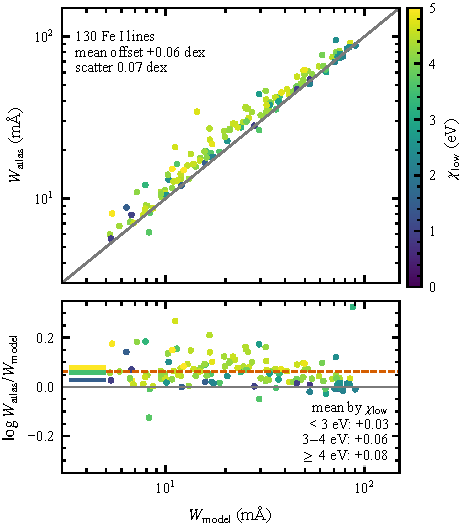
\includegraphics[width=\figwidth]{figures/validation.pdf}
\caption{Equivalent widths of 130 isolated solar \ion{Fe}{i} lines with laboratory oscillator strengths: measured in the Kitt Peak flux atlas \citep{Kurucz2005atlas} against computed with our code in the ATLAS9 solar model at $\log\epsilon_\mathrm{Fe} = 7.50$. Color gives the excitation energy of the lower level. Top: the gray line is equality. Bottom: logarithmic residuals; the dashed line is the mean, $+0.06$~dex, and the short bars are the means for lower levels below 3~eV, from 3 to 4~eV and above 4~eV.}
\label{fig:validation}
\end{figure}

\subsection{Detection threshold}
\label{sec:threshold}

We set the detection threshold on the equivalent width of a line whose position and shape are known, measured in a continuum-normalized spectrum with signal-to-noise ratio $S/N$ per pixel. A least-squares fit of a Gaussian profile of full width at half maximum $w$, sampled at pixel width $\Delta\lambda_\mathrm{pix}$, gives an equivalent width with standard error
\begin{equation}
\sigma_W = \frac{f_\mathrm{c}}{S/N} \left( \frac{w \, \Delta\lambda_\mathrm{pix}}{0.6643} \right)^{1/2} ,
\label{eq:sigmaw}
\end{equation}
where $0.6643 = (2\ln 2/\pi)^{1/2}$ is $w$ times the integral of the squared, unit-area Gaussian. This has the form of the classic estimate of \citet{Cayrel1988}; we include a factor $f_\mathrm{c} = 1.3$ for the uncertainty of the continuum placement. The observed width $w$ adds in quadrature the thermal and microturbulent Doppler width, macroturbulence, rotation (with full width $1.6\,v\sin i$) and the instrumental profile, and we take three pixels per resolution element. The lines of one species form a matched filter, so their significances add in quadrature,
\begin{equation}
Z = \left[ \sum_i \left( \frac{W_i}{\sigma_{W,i}} \right)^2 \right]^{1/2} ,
\label{eq:z}
\end{equation}
summed over the lines that fall within the instrument's wavelength coverage. We call the abundance at which $Z = 5$ the detection threshold. The \ion{Tc}{i} statistic uses the three resonance lines. The \ion{Tc}{ii} statistic uses the 41 lines with $\log gf \geq -1$ between 2000 and 10{,}000~\AA, and the \ion{Pm}{ii} statistic up to 40 lines (Table~\ref{tab:lines}).

We consider six representative instruments. The 8.2~m telescope with $R = 140{,}000$ over 3800--7880~\AA\ corresponds to ESPRESSO \citep{Pepe2021}. The others are generic: a 3.6~m telescope with $R = 115{,}000$ over 3780--6910~\AA, representative of the radial-velocity spectrographs on 4~m-class telescopes such as HARPS \citep{Mayor2003}; an ultraviolet-blue spectrograph on the 8.2~m telescope with $R = 80{,}000$ over 3050--5000~\AA; a 39~m telescope with $R = 100{,}000$ over 3500--18{,}000~\AA; a 2.4~m space telescope with an ultraviolet echelle at $R = 114{,}000$ over 1650--3100~\AA, the range of the near-ultraviolet detector of STIS \citep{Woodgate1998}; and a 6~m space telescope with $R = 100{,}000$ from 1000 to 10{,}000~\AA. The total efficiencies (telescope, spectrograph and detector) are round assumed values: 0.05 for the 3.6~m telescope, 0.08 for the 8.2~m and 39~m telescopes (ESPRESSO exceeds 10 percent at 5500~\AA; \citealt{Pepe2021}), 0.01 for the 2.4~m ultraviolet echelle and 0.05 for the 6~m telescope. They enter only the photon budget of Section~\ref{sec:horizon}. For a star of visual magnitude $V$ observed for a time $t$, the photon-limited signal-to-noise ratio per pixel at wavelength $\lambda$ is given by $(S/N)^2 = f_\lambda A \eta \Delta\lambda_\mathrm{pix} t \lambda / (hc)$, with $A$ the collecting area, $\eta$ the efficiency and $f_\lambda$ the flux density. We scale $f_\lambda$ from $f_\lambda(5500\,\mathrm{\AA}) = 3.77\times10^{-9} \times 10^{-0.4V}$~erg~s$^{-1}$~cm$^{-2}$~\AA$^{-1}$ by the line-blanketed flux of the ATLAS9 model nearest each host \citep{CastelliKurucz2003}, relative to its value at 5500~\AA. We derived that zero point from the solar model, the line blanketing of the solar atlas near 5500~\AA\ and $M_{V,\odot} = 4.79$ \citep{PecautMamajek2013}.

\subsection{Host stars}
\label{sec:hosts}

Table~\ref{tab:hosts} lists the seven hosts. Six span the main sequence from an M dwarf to an A0 star, with the Sun as the G-type host and an 8000~K star standing in for a slowly rotating Am star. The seventh is a quiet, slowly rotating late-B star of 12{,}250~K, like the HgMn stars, which mixes nothing below its atmosphere (Section~\ref{sec:levitation}). Absolute magnitudes are from the dwarf sequence of \citet{PecautMamajek2013}. Microturbulence is 1~km~s$^{-1}$ for the dwarfs cooler than 6000~K and for the late-B star, 1.5~km~s$^{-1}$ for the F dwarf and 2~km~s$^{-1}$ for the A stars. Projected rotation velocities are 2~km~s$^{-1}$ for the M and K dwarfs, 1.9~km~s$^{-1}$ for the Sun, 8~km~s$^{-1}$ for the F dwarf, 15~km~s$^{-1}$ for the A stars and 10~km~s$^{-1}$ for the late-B star. Macroturbulent widths are 1, 2, 3.5, 5, 3, 3 and 0~km~s$^{-1}$ in the same order. These values set the line widths that enter Equation~(\ref{eq:sigmaw}).

\begin{table}
\centering
\caption{Host stars. $M_\mathrm{mix}$ is the mass of the layer that the pollutant mixes into, with its adopted range in brackets (Section~\ref{sec:dilution}). The late-B star mixes only its atmosphere above $\tau_{5000} = 3$ (Section~\ref{sec:levitation}), and we give no range.}
\label{tab:hosts}
\footnotesize
\setlength{\tabcolsep}{3pt}
\begin{tabular}{lrrrrc}
\toprule
Host & $T_\mathrm{eff}$ (K) & $\log g$ & $M_\star$ ($M_\odot$) & $M_V$ & $\log(M_\mathrm{mix}/M_\odot)$ [range] \\
\midrule
M dwarf & 3500 & 5.00 & 0.40 & 10.48 & $-0.46$ [$-0.52$, $-0.40$] \\
K dwarf & 4500 & 4.50 & 0.70 & 7.17 & $-1.25$ [$-1.40$, $-1.10$] \\
Sun & 5777 & 4.44 & 1.00 & 4.79 & $-1.71$ [$-1.86$, $-1.56$] \\
F dwarf & 6250 & 4.50 & 1.25 & 3.88 & $-2.50$ [$-2.65$, $-2.35$] \\
Am star & 8000 & 4.00 & 1.80 & 2.07 & $-5.24$ [$-9.74$, $-4.74$] \\
A0 star & 9500 & 4.00 & 2.30 & 1.07 & $-5.14$ [$-9.64$, $-4.64$] \\
Late B & 12250 & 4.00 & 3.40 & 0.02 & $-10.06$ \\
\bottomrule
\end{tabular}

\end{table}

\section{Photospheric beacons}
\label{sec:results}

\citet{Whitmire1980} argued from the depth of the outer convection zone, without computing line strengths, that a polluted photosphere would be most visible in stars of types A5--F2. This section computes the beacon in each host of Table~\ref{tab:hosts}, tests that argument, and finds the cheapest photospheric beacon.

\subsection{Thresholds and inventories}
\label{sec:inventories}

Table~\ref{tab:budget} and Figure~\ref{fig:budget} give the detection threshold, the inventory from Equation~(\ref{eq:inventory}) and its energy cost for every host. Thresholds are for the 8.2~m, $R = 140{,}000$ instrument at $S/N = 300$, a routine value for a bright star, and for the 2.4~m ultraviolet echelle in the case of \ion{Tc}{ii}. At $S/N = 1000$ every threshold falls by 0.5~dex, and so does every inventory. These thresholds are for isolated lines. Synthesized among every line of other elements in Kurucz's lists at solar-scaled abundances, the Tc lines absorb less, because the other lines already remove part of the flux that they would absorb. The thresholds then rise by 0.28~dex in the Sun, 0.18~dex in the F dwarf, 0.13~dex in the Am star and 0.06~dex in the A0 and late-B stars, and $K$ by 0.006 to 0.03.

\begin{figure}[tb]
\centering
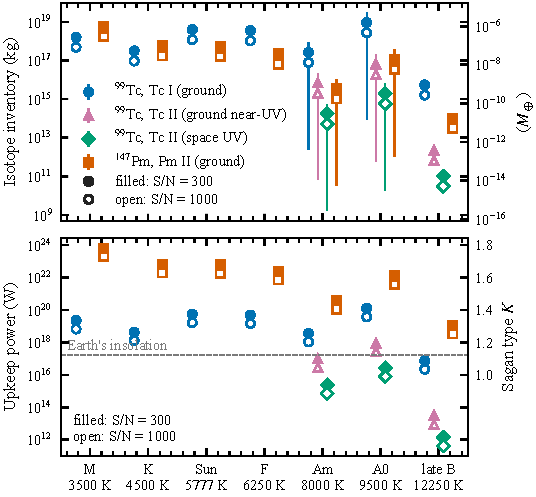
\includegraphics[width=\figwidth]{figures/budget.pdf}
\caption{Top: inventory of $^{99}$Tc and $^{147}$Pm that brings each host to a $5\sigma$ detection. Circles: \ion{Tc}{i} resonance lines from the ground (8.2~m, $R = 140{,}000$); triangles: \ion{Tc}{ii} near-ultraviolet lines from the ground (8.2~m, $R = 80{,}000$, A stars only); diamonds: \ion{Tc}{ii} ultraviolet lines from space (2.4~m, $R = 114{,}000$, A stars only); squares: \ion{Pm}{ii} from the ground. Filled symbols are for $S/N = 300$ per pixel, open symbols for $S/N = 1000$. Error bars span the adopted range of mixed mass; for the A stars it covers five orders of magnitude, and the late-B star has none. Bottom: upkeep power of Equation~(\ref{eq:upkeep}) for nuclides bred by neutron capture ($^{99}$Tc from $^{98}$Mo, $^{145}$Pm from $^{144}$Sm), with its Sagan type $K$ on the right axis. The dashed line is the sunlight intercepted by the Earth, $1.7\times10^{17}$~W \citep{Gray2020}. Below it lie the \ion{Tc}{ii} beacons of the Am and late-B stars, that of the A0 star read from space, and the \ion{Tc}{i} beacon of the late-B star.}
\label{fig:budget}
\end{figure}

\begin{table*}
\centering
\caption{Beacons that reach $Z = 5$ at $S/N = 300$ per pixel. Telescopes: 8.2~m with $R = 140{,}000$; 8.2~m ultraviolet-blue spectrograph with $R = 80{,}000$; 2.4~m space ultraviolet echelle with $R = 114{,}000$. The inventory is of $^{99}$Tc or $^{147}$Pm for the fiducial mixed mass. $K_\mathrm{fis}$ is the Sagan type of the upkeep when the nuclide is harvested from fission products ($^{99}$Tc, $^{147}$Pm). $P_\mathrm{up}$ and $K$ are the upkeep power of Equation~(\ref{eq:upkeep}) and its Sagan type when it is bred by neutron capture ($^{99}$Tc from $^{98}$Mo, $^{145}$Pm from $^{144}$Sm). For Pm the inventory is of $^{147}$Pm, but $P_\mathrm{up}$ and $K$ are for the same number of atoms of $^{145}$Pm. $^{235}$U: the mass fissioned to breed the inventory once. Target: the natural Mo (Sm for Pm) that holds the capture targets.}
\label{tab:budget}
\footnotesize
\setlength{\tabcolsep}{4pt}
\iftwocol\begin{tabular}{lllrrrrrrr}
\toprule
Host & Lines & Telescope & $\log\epsilon$ & Inventory (kg) & $K_\mathrm{fis}$ & $P_\mathrm{up}$ (W) & $K$ & $^{235}$U (kg) & Target (kg) \\
\midrule
M dwarf & Tc\,\textsc{i} & 8 m & $-1.49$ & $1.6\times10^{18}$ & 1.47 & $2.3\times10^{19}$ & 1.34 & $2.6\times10^{18}$ & $6.6\times10^{18}$ \\
 & Pm\,\textsc{ii} & 8 m & $-1.10$ & $5.9\times10^{18}$ & 2.05 & $6.6\times10^{23}$ & 1.78 & $6.5\times10^{18}$ & $1.9\times10^{20}$ \\
\addlinespace
K dwarf & Tc\,\textsc{i} & 8 m & $-1.41$ & $3.1\times10^{17}$ & 1.40 & $4.4\times10^{18}$ & 1.26 & $5.1\times10^{17}$ & $1.3\times10^{18}$ \\
 & Pm\,\textsc{ii} & 8 m & $-1.31$ & $5.9\times10^{17}$ & 1.95 & $6.6\times10^{22}$ & 1.68 & $6.4\times10^{17}$ & $1.9\times10^{19}$ \\
\addlinespace
Sun & Tc\,\textsc{i} & 8 m & $+0.16$ & $4.0\times10^{18}$ & 1.51 & $5.6\times10^{19}$ & 1.37 & $6.5\times10^{18}$ & $1.6\times10^{19}$ \\
 & Pm\,\textsc{ii} & 8 m & $-0.88$ & $5.4\times10^{17}$ & 1.94 & $6.1\times10^{22}$ & 1.68 & $6.0\times10^{17}$ & $1.7\times10^{19}$ \\
\addlinespace
F dwarf & Tc\,\textsc{i} & 8 m & $+0.89$ & $3.5\times10^{18}$ & 1.51 & $4.9\times10^{19}$ & 1.37 & $5.7\times10^{18}$ & $1.4\times10^{19}$ \\
 & Pm\,\textsc{ii} & 8 m & $-0.49$ & $2.2\times10^{17}$ & 1.90 & $2.5\times10^{22}$ & 1.64 & $2.4\times10^{17}$ & $7.0\times10^{18}$ \\
\addlinespace
Am star & Tc\,\textsc{i} & 8 m & $+2.51$ & $2.6\times10^{17}$ & 1.39 & $3.7\times10^{18}$ & 1.26 & $4.3\times10^{17}$ & $1.1\times10^{18}$ \\
 & Tc\,\textsc{ii} & 8 m, UV & $+0.93$ & $7.0\times10^{15}$ & 1.24 & $9.7\times10^{16}$ & 1.10 & $1.1\times10^{16}$ & $2.8\times10^{16}$ \\
 & Tc\,\textsc{ii} & 2.4 m, space & $-0.68$ & $1.7\times10^{14}$ & 1.08 & $2.4\times10^{15}$ & 0.94 & $2.8\times10^{14}$ & $7.0\times10^{14}$ \\
 & Pm\,\textsc{ii} & 8 m & $+0.45$ & $3.5\times10^{15}$ & 1.72 & $3.9\times10^{20}$ & 1.46 & $3.8\times10^{15}$ & $1.1\times10^{17}$ \\
\addlinespace
A0 star & Tc\,\textsc{i} & 8 m & $+3.94$ & $9.2\times10^{18}$ & 1.55 & $1.3\times10^{20}$ & 1.41 & $1.5\times10^{19}$ & $3.7\times10^{19}$ \\
 & Tc\,\textsc{ii} & 8 m, UV & $+1.79$ & $6.5\times10^{16}$ & 1.33 & $9.0\times10^{17}$ & 1.20 & $1.1\times10^{17}$ & $2.6\times10^{17}$ \\
 & Tc\,\textsc{ii} & 2.4 m, space & $+0.27$ & $1.9\times10^{15}$ & 1.18 & $2.7\times10^{16}$ & 1.04 & $3.1\times10^{15}$ & $7.9\times10^{15}$ \\
 & Pm\,\textsc{ii} & 8 m & $+1.86$ & $1.1\times10^{17}$ & 1.87 & $1.3\times10^{22}$ & 1.61 & $1.2\times10^{17}$ & $3.6\times10^{18}$ \\
\addlinespace
Late B & Tc\,\textsc{i} & 8 m & $+5.63$ & $5.4\times10^{15}$ & 1.23 & $7.5\times10^{16}$ & 1.09 & $8.8\times10^{15}$ & $2.2\times10^{16}$ \\
 & Tc\,\textsc{ii} & 8 m, UV & $+2.25$ & $2.2\times10^{12}$ & 0.89 & $3.1\times10^{13}$ & 0.75 & $3.7\times10^{12}$ & $9.1\times10^{12}$ \\
 & Tc\,\textsc{ii} & 2.4 m, space & $+0.91$ & $1.0\times10^{11}$ & 0.75 & $1.4\times10^{12}$ & 0.62 & $1.7\times10^{11}$ & $4.1\times10^{11}$ \\
 & Pm\,\textsc{ii} & 8 m & $+3.75$ & $1.0\times10^{14}$ & 1.57 & $1.2\times10^{19}$ & 1.31 & $1.1\times10^{14}$ & $3.3\times10^{15}$ \\
\bottomrule
\end{tabular}
\else\resizebox{\textwidth}{!}{\begin{tabular}{lllrrrrrrr}
\toprule
Host & Lines & Telescope & $\log\epsilon$ & Inventory (kg) & $K_\mathrm{fis}$ & $P_\mathrm{up}$ (W) & $K$ & $^{235}$U (kg) & Target (kg) \\
\midrule
M dwarf & Tc\,\textsc{i} & 8 m & $-1.49$ & $1.6\times10^{18}$ & 1.47 & $2.3\times10^{19}$ & 1.34 & $2.6\times10^{18}$ & $6.6\times10^{18}$ \\
 & Pm\,\textsc{ii} & 8 m & $-1.10$ & $5.9\times10^{18}$ & 2.05 & $6.6\times10^{23}$ & 1.78 & $6.5\times10^{18}$ & $1.9\times10^{20}$ \\
\addlinespace
K dwarf & Tc\,\textsc{i} & 8 m & $-1.41$ & $3.1\times10^{17}$ & 1.40 & $4.4\times10^{18}$ & 1.26 & $5.1\times10^{17}$ & $1.3\times10^{18}$ \\
 & Pm\,\textsc{ii} & 8 m & $-1.31$ & $5.9\times10^{17}$ & 1.95 & $6.6\times10^{22}$ & 1.68 & $6.4\times10^{17}$ & $1.9\times10^{19}$ \\
\addlinespace
Sun & Tc\,\textsc{i} & 8 m & $+0.16$ & $4.0\times10^{18}$ & 1.51 & $5.6\times10^{19}$ & 1.37 & $6.5\times10^{18}$ & $1.6\times10^{19}$ \\
 & Pm\,\textsc{ii} & 8 m & $-0.88$ & $5.4\times10^{17}$ & 1.94 & $6.1\times10^{22}$ & 1.68 & $6.0\times10^{17}$ & $1.7\times10^{19}$ \\
\addlinespace
F dwarf & Tc\,\textsc{i} & 8 m & $+0.89$ & $3.5\times10^{18}$ & 1.51 & $4.9\times10^{19}$ & 1.37 & $5.7\times10^{18}$ & $1.4\times10^{19}$ \\
 & Pm\,\textsc{ii} & 8 m & $-0.49$ & $2.2\times10^{17}$ & 1.90 & $2.5\times10^{22}$ & 1.64 & $2.4\times10^{17}$ & $7.0\times10^{18}$ \\
\addlinespace
Am star & Tc\,\textsc{i} & 8 m & $+2.51$ & $2.6\times10^{17}$ & 1.39 & $3.7\times10^{18}$ & 1.26 & $4.3\times10^{17}$ & $1.1\times10^{18}$ \\
 & Tc\,\textsc{ii} & 8 m, UV & $+0.93$ & $7.0\times10^{15}$ & 1.24 & $9.7\times10^{16}$ & 1.10 & $1.1\times10^{16}$ & $2.8\times10^{16}$ \\
 & Tc\,\textsc{ii} & 2.4 m, space & $-0.68$ & $1.7\times10^{14}$ & 1.08 & $2.4\times10^{15}$ & 0.94 & $2.8\times10^{14}$ & $7.0\times10^{14}$ \\
 & Pm\,\textsc{ii} & 8 m & $+0.45$ & $3.5\times10^{15}$ & 1.72 & $3.9\times10^{20}$ & 1.46 & $3.8\times10^{15}$ & $1.1\times10^{17}$ \\
\addlinespace
A0 star & Tc\,\textsc{i} & 8 m & $+3.94$ & $9.2\times10^{18}$ & 1.55 & $1.3\times10^{20}$ & 1.41 & $1.5\times10^{19}$ & $3.7\times10^{19}$ \\
 & Tc\,\textsc{ii} & 8 m, UV & $+1.79$ & $6.5\times10^{16}$ & 1.33 & $9.0\times10^{17}$ & 1.20 & $1.1\times10^{17}$ & $2.6\times10^{17}$ \\
 & Tc\,\textsc{ii} & 2.4 m, space & $+0.27$ & $1.9\times10^{15}$ & 1.18 & $2.7\times10^{16}$ & 1.04 & $3.1\times10^{15}$ & $7.9\times10^{15}$ \\
 & Pm\,\textsc{ii} & 8 m & $+1.86$ & $1.1\times10^{17}$ & 1.87 & $1.3\times10^{22}$ & 1.61 & $1.2\times10^{17}$ & $3.6\times10^{18}$ \\
\addlinespace
Late B & Tc\,\textsc{i} & 8 m & $+5.63$ & $5.4\times10^{15}$ & 1.23 & $7.5\times10^{16}$ & 1.09 & $8.8\times10^{15}$ & $2.2\times10^{16}$ \\
 & Tc\,\textsc{ii} & 8 m, UV & $+2.25$ & $2.2\times10^{12}$ & 0.89 & $3.1\times10^{13}$ & 0.75 & $3.7\times10^{12}$ & $9.1\times10^{12}$ \\
 & Tc\,\textsc{ii} & 2.4 m, space & $+0.91$ & $1.0\times10^{11}$ & 0.75 & $1.4\times10^{12}$ & 0.62 & $1.7\times10^{11}$ & $4.1\times10^{11}$ \\
 & Pm\,\textsc{ii} & 8 m & $+3.75$ & $1.0\times10^{14}$ & 1.57 & $1.2\times10^{19}$ & 1.31 & $1.1\times10^{14}$ & $3.3\times10^{15}$ \\
\bottomrule
\end{tabular}
}\fi
\end{table*}

The thresholds follow the ionization of the two elements. Technetium has an ionization energy of 7.1~eV. At $\tau_{5000} = 0.1$, where weak lines form, 99 percent of it is neutral in the M dwarf and 72 percent in the K dwarf, but only 4 percent in the Sun and less than 1 percent in the A stars. The \ion{Tc}{i} threshold therefore rises from $\log\epsilon = -1.5$ in the M dwarf and $-1.4$ in the K dwarf to $+0.2$ in the Sun, $+0.9$ in the F dwarf, $+2.5$ to $+3.9$ in the A stars and $+5.6$ in the late-B star. Promethium, with an ionization energy of 5.6~eV, is more than 98 percent singly ionized from the K dwarf to the F dwarf. Its 40 \ion{Pm}{ii} lines give a threshold between $\log\epsilon = -1.3$ and $-0.5$ across that range, which rises in the A stars as Pm becomes doubly ionized. In the A stars the \ion{Tc}{ii} resonance lines at 2543, 2610 and 2647~\AA\ are the most sensitive tracer of Tc, with thresholds of $\log\epsilon = -0.7$ (Am), $+0.3$ (A0) and $+0.9$ (late B) from space. From the ground, the \ion{Tc}{ii} lines at 3195, 3212 and 3237~\AA\ reach $\log\epsilon = +0.9$ (Am), $+1.8$ (A0) and $+2.3$ (late B) with the ultraviolet-blue spectrograph.

The inventory combines these thresholds with the mixed mass. A beacon of $^{99}$Tc in a Sun-like star needs $4\times10^{18}$~kg, or $7\times10^{-7}\,\Mearth$, to reach $Z = 5$ at $S/N = 300$. The K dwarf needs about ten times less, because its Tc is more neutral and its convection zone is only three times more massive. The M dwarf needs more than the K dwarf, because its convection zone holds nearly all of its mass. The F dwarf needs about the same as the Sun: its convection zone is six times lighter, but its Tc is more ionized. The A stars need far less, because their mixed layer is $10^{-5.5}$ of the stellar mass. The \ion{Tc}{ii} beacon in the Am star needs $1.7\times10^{14}$~kg and the \ion{Pm}{ii} beacon $3.5\times10^{15}$~kg, four orders of magnitude less than in the Sun. This confirms the argument of \citet{Whitmire1980} that hosts in the range A5--F2 are favored. It rests on the mixed mass of the Am star, which we take at the turbulent value. If only the hydrogen and helium convection zones mixed, the inventory would fall by another factor of $10^{4.5}$, but the abundances of Am stars require deeper mixing. The late-B star needs least of all, $1.0\times10^{11}$~kg from space and $2.2\times10^{12}$~kg from the ground, because the Tc fills only its atmosphere. Section~\ref{sec:levitation} gives the reasons for assuming that such a star mixes nothing below its atmosphere.

On the Kardashev scale (Section~\ref{sec:upkeep}) the ranking is the same. The cheapest detectable beacon is $^{99}$Tc in the late-B star: $1.4\times10^{12}$~W ($K = 0.62$) read from space, or $3.1\times10^{13}$~W ($K = 0.75$) read from the ground in the near-ultraviolet \ion{Tc}{ii} lines, which is still less than the Am beacon read from space. It rests on the assumption that the star mixes nothing below its atmosphere. Among the hosts whose mixing is known from their abundances, the cheapest is $^{99}$Tc in the Am star, read in the \ion{Tc}{ii} ultraviolet lines from space. Bred from $^{98}$Mo, its upkeep is $2.4\times10^{15}$~W, $K = 0.94$; harvested from fission products it would cost $K = 1.08$. Read from the ground in the near-ultraviolet \ion{Tc}{ii} lines, the same beacon needs $7.0\times10^{15}$~kg and $9.7\times10^{16}$~W ($K = 1.10$). Every Tc beacon in a dwarf from M to F costs $K = 1.26$--1.37, and every Pm beacon $K \geq 1.31$, because even $^{145}$Pm must be replaced every few decades. Breeding the longer-lived $^{97}$Tc from $^{96}$Ru instead would lower the upkeep of every Tc beacon by a further factor of 20 ($K = 0.81$ for the Am star), but its inventory would then take a half-life of 4.2~Myr to build at that power.

\subsection{Radiative support in A stars}
\label{sec:levitation}

The thin mixed layer of an A star keeps a beacon only if Tc does not sink out of it faster than it decays. Below the convection zones of an A star, an element settles unless the radiative acceleration on it, $g_\mathrm{rad}$, exceeds gravity \citep{Richer2000}. That acceleration is the momentum that the element's lines absorb from the outgoing flux, per unit mass of the element. We computed it for Tc in ATLAS9 models with $\log g = 4$ from 7000 to 14{,}000~K. We solved each line of \ion{Tc}{i}--\textsc{iii} with $\log gf > -3$ in its own frequency window. The opacity in the window includes the continuum, the line itself, the other Tc lines and the strong lines of 13 other elements from Kurucz's lists, so the acceleration falls as the lines saturate. Below 2000~\AA\ we scaled the flux to the blanketed fluxes of \citet{CastelliKurucz2003}, and we weighted the accelerations on the three ions by their diffusion coefficients. We take a microturbulence of 0.5~km~s$^{-1}$, as in a quiet atmosphere in which diffusion can act. Less turbulence saturates the lines more, so this choice is conservative.

We tested the method at 12{,}250~K, close to the 12{,}000~K model in which \citet{AlecianStift2019} follow the diffusion of Mg and Fe. At the solar abundance, Mg is supported only above $\tau_{5000} \approx 10^{-2}$ and not where its lines form, where $\log g_\mathrm{rad} = 3.2$--3.6. Fe is pushed upward at every depth, with $\log g_\mathrm{rad} = 5.1$--5.3. Both agree with their results. Mn is pushed upward even at 100 times its solar abundance ($\log g_\mathrm{rad} = 5.2$--5.3), as the large Mn excesses of HgMn stars of this temperature suggest \citep{SmithDworetsky1993}.

\begin{table}
\centering
\caption{Radiative acceleration on Tc relative to gravity, $\log(g_\mathrm{rad}/g)$, in ATLAS9 models with $\log g = 4$, at the depth between $\tau_{5000} = 10^{-4}$ and 3 where it is smallest. $\log\epsilon_\mathrm{Tc}$ is the threshold of the \ion{Tc}{ii} ultraviolet beacon (2.4~m space echelle, $S/N = 300$) for a star rotating at $v\sin i = 10$~km~s$^{-1}$. Unsaturated: each line in the continuum flux at the threshold abundance. Threshold and $100\times$ threshold: every line solved in its own window at those abundances.}
\label{tab:levitation}
\footnotesize
\setlength{\tabcolsep}{4pt}
\begin{tabular}{rrrrr}
\toprule
$T_\mathrm{eff}$ (K) & $\log\epsilon_\mathrm{Tc}$ & Unsaturated & Threshold & $100\times$ threshold \\
\midrule
7000 & $-1.33$ & 1.35 & 1.14 & 0.74 \\
8000 & $-0.76$ & 1.43 & 1.31 & 1.01 \\
9000 & $-0.10$ & 1.53 & 1.47 & 1.26 \\
10000 & $+0.39$ & 1.71 & 1.68 & 1.50 \\
11000 & $+0.67$ & 1.90 & 1.86 & 1.70 \\
12250 & $+0.91$ & 2.12 & 2.05 & 1.90 \\
14000 & $+1.38$ & 2.50 & 2.33 & 2.00 \\
\bottomrule
\end{tabular}

\end{table}

Table~\ref{tab:levitation} gives the result for Tc. At the threshold of the \ion{Tc}{ii} space beacon, radiation pushes Tc upward 14 times harder than gravity pulls it down at 7000~K, and more than 200 times harder at 14{,}000~K, at every depth from $\tau_{5000} = 10^{-4}$ to 3. Saturation lowers the acceleration by at most 0.2~dex at the threshold, and at 100 times the threshold radiation still pushes 5 times harder than gravity. Technetium is therefore pushed upward throughout the atmosphere of an A star. The mixed layer of the Am star, however, reaches down to $\log(\Delta M/M_\star) = -5.5$, where Tc is highly ionized and these accelerations do not apply. Tc leaves the layer through its base, where turbulence gives way to diffusion, and it would leave slowly even with no radiative support there. \citet{Richard2001} find 200{,}000~K at $\log(\Delta M/M_\star) \approx -6.5$ in A stars, and a radiative envelope then puts the base of the layer at $T \approx 3$--$4\times10^{5}$~K. For Tc ten times ionized, collisions with protons limit its settling to about $2\times10^{-6}$~cm~s$^{-1}$, and the layer empties in $8\times10^{7}$~yr. For temperatures up to $10^{6}$~K and charges from 6 to 16 it takes no less than $1\times10^{7}$~yr, 50 half-lives. Decay therefore sets the lifetime of the beacon, and the upkeep of Section~\ref{sec:upkeep} holds for A stars as for FGK dwarfs. The abundances of Am stars require separation at $\log(\Delta M/M_\star) \approx -6$ to $-5$ \citep{Vick2010}, so an Am star mixes far below its convection zones, and over that range its \ion{Tc}{ii} space beacon costs $K = 0.89$ to 0.99. A quieter host does better. The non-magnetic HgMn stars are late-B stars whose atmospheres are modeled with diffusion acting against only a weak wind \citep{AlecianStift2019}. We take such a star at 12{,}250~K and $\log g = 4$, with the 3.4~$\Msun$ that \citet{AlecianStift2019} derive for these parameters, rotating at $v\sin i = 10$~km~s$^{-1}$. If it mixes nothing below its atmosphere, the beacon fills only the layer above $\tau_{5000} = 3$, which holds $10^{-10.6}$ of the stellar mass. It then needs $1\times10^{11}$~kg of $^{99}$Tc and an upkeep of $1.4\times10^{12}$~W ($K = 0.62$). A wind of $1.7\times10^{-14}\,\Msun$~yr$^{-1}$, the lowest rate with which \citet{AlecianStift2019} fit Mg and Fe, replaces that layer in 5000~yr and carries the Tc with it. Replacing that loss raises the upkeep to $9\times10^{13}$~W ($K = 0.79$).

A star that does not mix also does nothing to keep the Tc in its atmosphere. An ion that radiation pushes upward drifts through the hydrogen at a speed set by its collisions with protons and hydrogen atoms. At the threshold abundance, Tc drifts upward at about 1~cm~s$^{-1}$ at $\tau_{5000} = 1$ and 60~cm~s$^{-1}$ at $\tau_{5000} = 2\times10^{-4}$. It crosses the 15{,}000~km of atmosphere above $\tau_{5000} = 3$ in 11~yr. In the models of \citet{AlecianStift2019}, mass loss lets the elements that radiation pushes much harder than gravity escape from the top of the atmosphere, and only a weak horizontal magnetic field makes them accumulate. If the Tc escapes, the beacon must be refilled every 11~yr instead of once per mean life. Its upkeep then rises to $4\times10^{16}$~W ($K = 1.06$), more than that of the Am star. A horizontal field holds an ion only where the ion circles the field lines faster than it collides with the gas. For Tc this takes about 30~G at $\tau_{5000} = 10^{-5}$ and 3~kG at $\tau_{5000} = 10^{-2}$. HgMn stars show no large-scale field at a precision of 3--6~G, and no tangled field stronger than a few hundred gauss \citep{Kochukhov2013}. Fields far weaker than these limits have been found in other quiet stars: line-of-sight fields of $-0.6$~G in Vega and 0.2~G in Sirius~A \citep{Lignieres2009, Petit2011}, and in the Am stars $\beta$~UMa and $\theta$~Leo fields about a hundred times weaker than those of the weakest Ap stars \citep{Blazere2016}. A large-scale horizontal field of a few tens of gauss would probably show in the circular polarization that sets the 3--6~G limits, but a tangled field of that strength would not. A tangled field holds Tc only where it is close to horizontal, and lets it escape along the field elsewhere, so only part of the surface could hold a beacon. Where it does, a field of a few tens of gauss keeps the Tc only above $\tau_{5000} \approx 10^{-5}$. Held there, the same column of Tc gives \ion{Tc}{ii} ultraviolet lines 4 to 12 times stronger than when it fills the atmosphere evenly. Above $\tau_{5000} = 0.1$ most Tc is singly ionized, whereas at $\tau_{5000} = 1$ almost all of it is doubly ionized, and the cooler gas there also deepens the lines. Concentrated in that layer, the Tc reaches $\log\epsilon = 4.9$, and radiation still pushes it upward 20 times harder than gravity, so its own lines do not saturate enough to let it sink. Such a beacon would cost no more than $K = 0.62$. These layers are far from LTE, however, and this case is the least certain of our results. We therefore take $K = 1.06$ as the cost of the late-B beacon, and $K = 0.62$ or less as its cost if a weak field holds the Tc. The kilogauss fields of magnetic Ap stars would hold Tc even in the layers where its lines form, but these fields are mostly dipoles \citep{Kochukhov2019}. Radiation pushes the Tc along the field lines, out of the atmosphere into the magnetosphere at all but the lowest magnetic latitudes, and within 3 to 180~yr into a thin sheet at the magnetic equator. We therefore do not consider Ap stars as hosts.

The calculation is in LTE and does not redistribute the absorbed momentum when an ion changes stage. For \ion{Tc}{ii} it uses only lines between measured levels, which underestimates the acceleration. It does not follow the diffusion of Tc in time, so it shows which way Tc moves but not where it accumulates. An abundance that rises outward would strengthen or weaken the lines from which the thresholds are derived, depending on where they form.

\subsection{The beacon in a real spectrum}
\label{sec:blending}

The thresholds above assume isolated lines and an observer who knows the star's spectrum to the photon noise. Real spectra are crowded. In the Sun, none of the three \ion{Tc}{i} resonance lines lies on clean continuum: within 0.05~\AA\ of line center the solar flux atlas \citep{Kurucz2005atlas} drops to 0.83, 0.82 and 0.31 of the continuum at 4238, 4262 and 4297~\AA. Of the 40 \ion{Pm}{ii} lines, 15 have atlas flux above 0.9 within 0.05~\AA, and using only those raises the Pm threshold in the Sun by a factor of 12 in inventory. Figure~\ref{fig:spectrum} shows the cheapest beacon, \ion{Tc}{ii} in a quiet late-B star, in the best archival spectrum of such a star, the STIS E230H spectrum of the HgMn star HD~175640. Of its 11 Tc lines, 3 lie on clean continuum, which we take as flux above 0.9 of the continuum within half a line width of line center. The strongest line, at 2543~\AA, sits in the wing of a blend, and the line at 2610~\AA\ in a deep one. We measured how much Tc an observer would detect with the clean lines alone. We added Tc to the archival spectrum and compared the absorption at the clean Tc lines with the same measurement at 400 equally clean places within 20~\AA\ of each line, so that the noise includes the weak lines of the star. In HD~175640 a $5\sigma$ detection then needs $\log\epsilon = 2.4$, whereas photon noise alone with every line would allow 0.8, a factor of 40 in inventory and 0.16 in $K$. The archival spectrum has a median $S/N$ of 110 per pixel. Degraded to $S/N = 31$, it needs almost as much with the clean lines, $\log\epsilon = 2.5$, because the weak lines of the star, not photon noise, limit them; photon noise alone would then allow 1.5, so the penalty falls to a factor of 10. We ran the same test on the archival spectra of Section~\ref{sec:archival}, leaving out IUE, whose resolution leaves almost no line clean. For 218 stars, the clean-line detection lies a median 0.9~dex above the archival limit in the late-B and A stars and 0.2~dex above it in the FGK and horizontal-branch stars. The comparison must be local. Drawn from the whole spectrum, it puts the Tc lines of 34 stars, most of them metal-poor, $5\sigma$ or more below the clean continuum before any Tc is added, because the Tc lines lie in the crowded blue and ultraviolet. Drawn within 20~\AA, it leaves no spectrum above $4.3\sigma$.

\begin{figure*}[t]
\centering
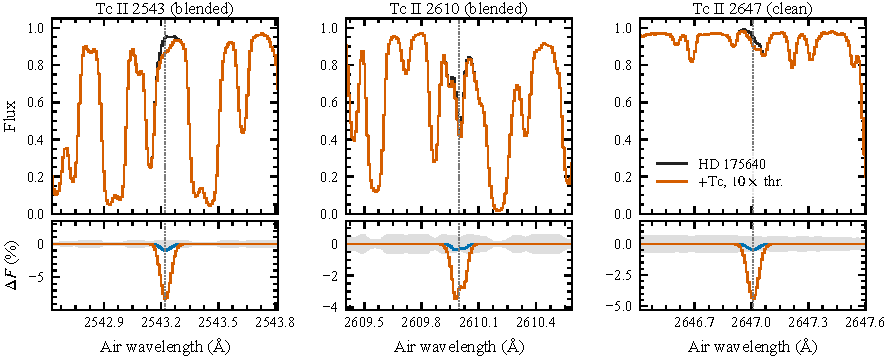
\includegraphics[width=\textwidth]{figures/spectrum.pdf}
\caption{The beacon in a real spectrum. Top: the HST STIS E230H spectrum of the HgMn star HD~175640 near three \ion{Tc}{ii} lines (black), and the same spectrum with Tc added at ten times the $5\sigma$ threshold abundance of the late-B host read from space, $\log\epsilon = 1.9$ (orange). Line profiles are computed in the star's own model atmosphere. Bottom: the change in flux, in percent of the continuum, at the threshold (blue) and at ten times the threshold (orange), and the per-pixel noise of the spectrum (gray band). Dotted lines mark the Tc lines; only the line at 2647~\AA\ lies on clean continuum. The threshold is set by all the lines together, so each line at threshold lies below the per-pixel noise.}
\label{fig:spectrum}
\end{figure*}

The thresholds of Table~\ref{tab:budget} therefore assume a receiver that knows the star's own spectrum to the photon noise, so that every Tc line counts, blended or not. A beacon must be found differentially, by comparing the target with a spectrum that has no beacon: the same star at an earlier epoch, a spectroscopic twin, or a synthetic spectrum good to a fraction of a percent. That comparison, not photon noise, will usually set the limit. Today's synthetic spectra fall far short of it in the ultraviolet. We fitted an LTE synthesis to the STIS spectrum of HD~175640 within 3~\AA\ of each Tc line, with the Kurucz lines of every element from Li to U, a free abundance for each element, a free line width and a free continuum. The fit recovers the abundances of Mn, Ti, Cr and Fe found by \citet{Castelli2015} to within 0.3~dex, but it misses the spectrum by 9 to 14 percent of the continuum, 20 to 42 times the photon noise. An observer who divided the spectrum by this model and used every Tc line would detect Tc only at $\log\epsilon = 3.3$, which is worse than with the clean lines alone. \citet{Castelli2015} fitted the same spectrum with a model atmosphere made for the star, lines of 14 heavy ions added by hand, predicted lines and tuned abundances, and still found numerous unidentified lines between 2380 and 2700~\AA, where the \ion{Tc}{ii} lines lie. What limits these models is missing energy levels and lines, uncertain oscillator strengths, abundances that change with depth, and the assumption of LTE. These are gaps in knowledge, not limits set by physics, and a receiver that closes them reaches the thresholds of Table~\ref{tab:budget}. Until then the practical threshold is the clean-line one, 40 times the ideal inventory in HD~175640. This is why Section~\ref{sec:horizon} caps the effective signal-to-noise ratio at $S/N = 1000$.

\subsection{A radium beacon}
\label{sec:radium}

Radium is the only other element with no stable isotope whose singly ionized lines have known transition probabilities. In an FGK dwarf most of its atoms are in Ra~\textsc{ii}, whose resonance line at 3814~\AA\ is strong. We computed the threshold of a photospheric $^{226}$Ra beacon with the same hosts, telescopes and detection rule as for Tc, using the NIST transition probabilities and partition functions summed over the NIST levels of Ra~\textsc{i} and Ra~\textsc{ii} \citep{NIST2024}. In the Sun, read from the ground at $S/N = 300$, the beacon reaches $Z = 5$ at $\log\epsilon_\mathrm{Ra} = -2.45$. That is 2.6~dex below the \ion{Tc}{i} threshold, so the inventory is 180 times smaller, $2.2\times10^{16}$~kg. In the Am star it needs $2\times10^{14}$~kg, about as much as the \ion{Tc}{ii} beacon, but it is read from the ground rather than from space.

A radium beacon needs no fission. $^{226}$Ra has no route from a stable target, but a stock of natural uranium in secular equilibrium makes it as fast as the radium in the star decays. That stock must hold $3.0\times10^{6}$ times the inventory (Table~\ref{tab:nuclides}): $7\times10^{22}$~kg of uranium for the Sun, 1 percent of the Earth's mass. That is 100 times more uranium than the \ion{Tc}{i} beacon burns over a whole half-life of $^{99}$Tc, and in the Am star the ratio is $2\times10^{4}$. Ra~\textsc{ii}~3814 also lies in a deep blend in the Sun. With only the clean lines at 7078 and 8020~\AA\ the solar threshold rises to $\log\epsilon_\mathrm{Ra} = +0.30$. A radium beacon thus trades the power of a Tc beacon for a planet's worth of uranium, and we do not consider it further.

Even in the Am star, the beacon must fill a layer that holds $10^{-5.5}$ of the stellar mass, far more than the layers in which the lines form. Section~\ref{sec:gas} asks how much less a beacon needs when the dopant is placed in front of the star instead.

\section{Gas in front of the star}
\label{sec:gas}

Every atom of a dopant between a star and its observer absorbs. The young A star $\beta$~Pictoris shows variable, Doppler-shifted absorption in its Ca\,\textsc{ii} H and K lines \citep{Kiefer2014} and in many ultraviolet lines of Fe\,\textsc{ii} \citep{Vrignaud2024a}, from gas that evaporates from comets as they transit the star, and some twenty stars are now known to show similar features \citep{Rebollido2020}. A civilization could mix a radionuclide into such a comet. We modeled the absorption with the cloud of \citet{Vrignaud2024a}, which covers a fraction $\alpha$ of the stellar disk and spreads over a radial-velocity interval $\Delta v$, with its levels populated at the stellar $T_\mathrm{eff}$ \citep{Vrignaud2024b}. We calibrated it on the comet that transited $\beta$~Pic on 1997 December 6 ($\alpha = 0.4$, $\Delta v = 28$~km~s$^{-1}$, an Fe\,\textsc{ii} column of $1.1\times10^{15}$~cm$^{-2}$), assumed that the dopant is singly ionized like Fe and Ca, and added the significances of its lines as in Equation~(\ref{eq:z}). As a check, the Cr\,\textsc{ii} column measured in that comet is ten times our $5\sigma$ threshold at $S/N = 100$, which the ultraviolet spectra of $\beta$~Pic reach in long exposures \citep{Vrignaud2024a}.

Radium is the easiest dopant to detect. $^{226}$Ra lives 1600~yr, long enough to survive a comet's infall, and \ion{Ra}{ii} has the structure of Ca\,\textsc{ii}, with a resonance doublet at 3814 and 4682~\AA\ \citep{NIST2024}. A 3.6~m telescope at $S/N = 300$ detects it at a column of $4.4\times10^{10}$~cm$^{-2}$, as easily as Ca\,\textsc{ii} and at $4\times10^{-5}$ of the comet's iron; \ion{Tc}{ii} needs $1.9\times10^{11}$~cm$^{-2}$ in its ultraviolet resonance lines from space. A comet releases its refractory material only within several tens of stellar radii \citep{Kiefer2019}, so a $\beta$~Pic-like comet around our Am host has only 2 percent of its dopant in front of the star during a transit. We cost a gas beacon by the rate of events that gives a monitoring program an even chance of catching at least one in 10~yr. Each event is caught with probability $1 - \exp(-nt)$, for $n$ spectra a year taken at random and an event that stays detectable for a time $t$. A program from the ground takes 530 spectra a year, as many as HARPS has taken of $\beta$~Pic \citep{Hoeijmakers2025}; a program in space, 20. A $\beta$~Pic-like comet doped with $^{99}$Tc and read from space then costs $K = 1.20$. Releasing the dopant only during the transit, and slowly enough that it spreads over 3~km~s$^{-1}$ instead of 28~km~s$^{-1}$, lowers this to $K = 0.99$, about the cost of the photospheric beacon in the same star. A 90 percent chance instead of an even one raises the cost of every gas beacon by 0.05 in $K$. Radium cannot be bred from a stable target, and each kilogram must be extracted from $3.0\times10^{6}$~kg of natural uranium, so a radium comet is limited by the supply of uranium rather than by energy.

Around a Sun-like star a civilization can do better without a comet. It can release a cloud of neutral $^{99}$Tc at rest on the line of sight from its star to a chosen target, which we call an artificial comet. Ions would not serve, because the stellar wind picks up an ion within about one gyroperiod \citep{Gaffey1988} and carries it away at several hundred km~s$^{-1}$ \citep{Woch1997}. Radiation pressure on neutral Tc exceeds gravity by a factor of about 10 and pushes the cloud along the line of sight, so the cloud stays on the stellar disk while it recedes. Far from the star only the ground level is populated, and every atom absorbs in the \ion{Tc}{i} resonance lines, which are seen from the ground. The cloud is lost when it spreads sideways off the disk, after about 60~d for gas released at 100~K, or when it is photoionized. We take the photoionization rate of the homologue Mn \citep{Heays2017}, which gives a lifetime of 53~d at 1~AU that grows as $r^{2}$. Each cloud holds $4\times10^{7}$~kg. A cloud that stays on the disk for more than a day is almost certain to be caught by the ground-based program, so one cloud every 13~yr gives it an even chance in 10~yr. That costs $1.3\times10^{13}$~W ($K = 0.71$), whatever the release distance beyond 0.2~AU and the release temperature. Beyond about 2.5~AU the cloud outlives its spreading time of two months, and a cloud kept on there continuously costs $K = 0.90$. Moving the dopant into place costs less than $4\times10^{-5}$ of breeding it. The cloud covers the disk only for observers within $0.1^\circ$ of its line of sight, so it is aimed at one system at a time. As radiation pressure accelerates it, its lines drift blueward by about 0.6~km~s$^{-1}$ a day.

A civilization that does not know where its audience lives can release the gas as a belt or a shell instead. Seen from the host, most of the stars of the Galaxy lie at low Galactic latitude $b$: in a model of the Galaxy with the structure of \citet{BlandHawthorn2016}, half lie within $1.3^\circ$ of the plane. A belt released at 0.22~AU that serves observers at $|b| < 3^\circ$ covers 76 percent of the stars for $K = 1.02$, and a shell seen from every direction costs $K = 1.12$. Both are released close to the star, where the gas accelerates fast enough to smear its lines within a long exposure, so a 39~m telescope sees them in one 15-minute exposure only out to about 300~pc. Most of the stars that a belt covers are kiloparsecs away, and seeing it from there takes a larger telescope or a search that adds exposures along trial accelerations.

\section{Archival limits on technetium}
\label{sec:archival}

The thresholds of Section~\ref{sec:results} say how much Tc a beacon needs in order to be seen. Public archives already hold high-resolution spectra of many stars that would make good hosts, so they show how much Tc those stars could hold without our noticing. We collected the archival spectra of 222 such stars and set an upper limit on $\log\epsilon_\mathrm{Tc}$ in each. None of them shows Tc.

\subsection{Sample and method}
\label{sec:archival_method}

The stars are of the kinds that the previous sections favor as hosts, and each has published atmospheric parameters. They are the HgMn, Am and Ap stars of the compilation of \citet{Ghazaryan2018} that rotate at $v\sin i \leq 30$~km~s$^{-1}$, slowly rotating late-B stars with normal abundances, and slowly rotating metal-poor dwarfs and horizontal-branch stars. Of the 222, 45 are HgMn stars, 22 are Am stars, 73 are Ap or Bp stars, 38 have normal abundances, 35 are metal-poor dwarfs and subgiants, 8 lie on the horizontal branch, and the type of one, HD~27749, is uncertain. The parameters of every star and their sources, the spectra used and the limits are listed in the machine-readable table \texttt{archival\_limits.csv} that accompanies this paper. The ultraviolet spectra are from the HST STIS and GHRS echelles and from IUE, and the optical spectra from UVES, HARPS, FEROS, ESPRESSO, ELODIE, SOPHIE, ESPaDOnS and Narval. We left out four stars whose spectra contain a second star.

For each instrument we shifted every exposure to rest with the peak of its cross-correlation against a mask of the star's strongest lines. We kept the exposures whose peak stands $4\sigma$ above the rest of the cross-correlation, and averaged them with inverse-variance weights. We used every \ion{Tc}{i} and \ion{Tc}{ii} line between 1850 and 7000~\AA\ whose equivalent width at $\log\epsilon_\mathrm{Tc} = 3$ exceeds 5~m\AA\ in the star's model, and at least the ten strongest lines that each spectrum covers. Table~\ref{tab:lines} marks the lines that set a limit, and the machine-readable table \texttt{tc\_lines.csv} lists all 219 of them. For each line we then synthesized the Tc line alone (Section~\ref{sec:synthesis}), broadened to the width of the star's cross-correlation, in the ATLAS9 model nearest the star. For metal-poor and horizontal-branch stars the model comes from the grid nearest their [Fe/H] \citep{CastelliKurucz2003}, with the $\alpha$ elements enhanced at [Fe/H]~$\leq -1$. We divided each stack by its upper envelope, the 97th percentile of its flux in a running 10~\AA\ window, and placed the synthetic line on that envelope. The limit is the largest abundance at which the Tc line stays above the observed spectrum minus three times its noise, within half a line width of line center. This is a one-sided 99.87 percent criterion in each pixel, not a confidence level for the line as a whole, and it is not the statistic with which we detect lines (Section~\ref{sec:archival_search}). We did not model the rest of the spectrum, so any blend at a Tc wavelength counts against Tc and makes the limit conservative.

Because the model omits metal bound-free opacity (Section~\ref{sec:limitations}), it can make lines too deep. We therefore multiplied the continuum opacity by 1, 3 or 10, and kept the smallest factor at which the model's unsaturated Fe lines, at the star's published Fe abundance, are no deeper than the observed ones. Of the 222 stars, 183 need no correction and 17 need a factor of 3 or 10. The other 22 have no published Fe, and we left them uncorrected.

\subsection{Limits by host class}
\label{sec:archival_results}

A limit on $\log\epsilon_\mathrm{Tc}$ becomes a limit on the inventory once the mass that the Tc fills is fixed (Section~\ref{sec:dilution}). We take that mass from the host class of each star, as in Section~\ref{sec:results}. The 72 HgMn and normal late-B stars are quiet late-B hosts, whose Tc stays in the atmosphere above $\tau_{5000} = 3$ (Section~\ref{sec:levitation}). We assign the other classes by the star's type, not its temperature. The 103 Am, Ap and Bp stars and other stars hotter than 6400~K mix a turbulent layer that holds $10^{-5.5}$ of their mass. We give the 8 horizontal-branch stars the same layer, but it was calibrated on models of main-sequence stars, so their $K$ is only indicative. The 39 metal-poor and normal dwarfs mix their convection zone, which we take from the solar-metallicity models of \citet{Pinsonneault2001} at the star's temperature, or at 6400~K for the three metal-poor dwarfs that are hotter. A metal-poor star may have a thinner convection zone than these models give, and then a lower $K$. We compared each limit with the threshold that the same star would have at $S/N = 300$, computed in its own model with its own rotation: \ion{Tc}{i} from the ground for the dwarfs that mix their convection zone, and \ion{Tc}{ii} from space for the others. Their difference, $\Delta K = (\log\epsilon_\mathrm{limit} - \log\epsilon_\mathrm{threshold})/10$, does not depend on the mixed mass. The radii are from Gaia DR3 \citep{Creevey2023}, or, for 73 stars, from $V$, the parallax and the bolometric corrections of \citet{Torres2010}. Table~\ref{tab:archival} lists the lowest limits of each class, and Figure~\ref{fig:archival} shows all of them as the Sagan type of the upkeep that the largest allowed inventory would need.

\begin{table*}[t]
\centering
\caption{The lowest archival limits of each host class. $\log\epsilon_\mathrm{Tc}$ is the upper limit, set by the line and instrument listed. Threshold: the abundance that the same star would show at $Z = 5$ and $S/N = 300$ in its own model (Section~\ref{sec:archival_results}). $K$ is the Sagan type of the upkeep of the largest inventory that the limit allows, when the Tc fills the mixed mass of the star's class. $\Delta K = (\log\epsilon_\mathrm{Tc} - \mathrm{threshold})/10$; a negative $\Delta K$ means that the spectrum already excludes the beacon that the star would show at threshold.}
\label{tab:archival}
\footnotesize
\setlength{\tabcolsep}{4pt}
\iftwocol\begin{tabular}{llrrrlrr}
\toprule
Star & Type & $T_\mathrm{eff}$ (K) & $\log\epsilon_\mathrm{Tc}$ & Threshold & Line, instrument & $K$ & $\Delta K$ \\
\midrule
\multicolumn{8}{l}{\emph{Quiet late-B hosts (atmosphere)}} \\
HD~175640 & HgMn & 12000 & $\leq +1.7$ & $+0.6$ & Tc\,\textsc{ii} 2543, STIS E230H & 0.69 & $+0.11$ \\
HD~144667 & HgMn & 13990 & $\leq +2.3$ & $+1.2$ & Tc\,\textsc{ii} 2543, STIS E230H & 0.70 & $+0.11$ \\
HD~215573 & normal & 14050 & $\leq +2.3$ & $+1.3$ & Tc\,\textsc{ii} 2543, STIS E230H & 0.78 & $+0.10$ \\
53 Tau & HgMn & 11900 & $\leq +3.1$ & $+0.7$ & Tc\,\textsc{ii} 3237, UVES & 0.80 & $+0.24$ \\
$\chi$~Lup~A & HgMn & 10650 & $\leq +2.9$ & $+0.4$ & Tc\,\textsc{ii} 2647, GHRS G270M & 0.80 & $+0.25$ \\
\addlinespace
\multicolumn{8}{l}{\emph{Am and Ap stars (turbulent layer)}} \\
HD~213637 & Ap/Bp & 6400 & $\leq +2.0$ & $-1.9$ & Tc\,\textsc{i} 4096, ESPaDOnS & 1.15 & $+0.39$ \\
HD~114330 & Am & 9600 & $\leq +2.5$ & $-0.1$ & Tc\,\textsc{ii} 3237, UVES & 1.18 & $+0.26$ \\
$\eta$~Lep & normal & 6989 & $\leq +2.0$ & $-1.2$ & Tc\,\textsc{ii} 3237, UVES & 1.20 & $+0.32$ \\
32 Aqr & Am & 7700 & $\leq +1.9$ & $-1.1$ & Tc\,\textsc{ii} 3237, UVES & 1.20 & $+0.30$ \\
HD~172167 & Am & 9400 & $\leq +1.8$ & $+0.3$ & Tc\,\textsc{ii} 2647, STIS E230H & 1.21 & $+0.15$ \\
\addlinespace
\multicolumn{8}{l}{\emph{Horizontal-branch stars (turbulent layer, uncalibrated)}} \\
HD~161817 & BHB & 7400 & $\leq +0.5$ & $-1.3$ & Tc\,\textsc{ii} 2647, STIS E230M & 0.98 & $+0.18$ \\
HD~86986 & BHB & 7980 & $\leq +1.2$ & $-1.0$ & Tc\,\textsc{ii} 2543, STIS E230H & 1.04 & $+0.22$ \\
HD~74721 & BHB & 8810 & $\leq +1.4$ & $-0.7$ & Tc\,\textsc{ii} 2647, STIS E230M & 1.07 & $+0.21$ \\
HD~93329 & BHB & 8180 & $\leq +2.3$ & $-0.8$ & Tc\,\textsc{ii} 3237, UVES & 1.15 & $+0.31$ \\
HD~128801 & BHB & 10300 & $\leq +3.0$ & $+0.3$ & Tc\,\textsc{ii} 3237, UVES & 1.25 & $+0.27$ \\
\addlinespace
\multicolumn{8}{l}{\emph{FGK stars (convection zone)}} \\
HD~84937 & metal-poor & 6340 & $\leq +0.5$ & $+0.7$ & Tc\,\textsc{i} 4032, ESPRESSO & 1.30 & $-0.02$ \\
BD$-$10 388 & metal-poor & 6350 & $\leq +0.8$ & $+0.7$ & Tc\,\textsc{i} 4032, ESPRESSO & 1.33 & $+0.02$ \\
HD~140283 & metal-poor & 5762 & $\leq -0.1$ & $+0.1$ & Tc\,\textsc{i} 4032, ESPaDOnS & 1.35 & $-0.02$ \\
BD$-$04 3208 & metal-poor & 6330 & $\leq +1.0$ & $+0.5$ & Tc\,\textsc{i} 4032, ESPRESSO & 1.36 & $+0.05$ \\
HD~338529 & metal-poor & 6351 & $\leq +1.2$ & $+0.7$ & Tc\,\textsc{i} 4032, UVES & 1.37 & $+0.05$ \\
\bottomrule
\end{tabular}
\else\resizebox{\textwidth}{!}{\begin{tabular}{llrrrlrr}
\toprule
Star & Type & $T_\mathrm{eff}$ (K) & $\log\epsilon_\mathrm{Tc}$ & Threshold & Line, instrument & $K$ & $\Delta K$ \\
\midrule
\multicolumn{8}{l}{\emph{Quiet late-B hosts (atmosphere)}} \\
HD~175640 & HgMn & 12000 & $\leq +1.7$ & $+0.6$ & Tc\,\textsc{ii} 2543, STIS E230H & 0.69 & $+0.11$ \\
HD~144667 & HgMn & 13990 & $\leq +2.3$ & $+1.2$ & Tc\,\textsc{ii} 2543, STIS E230H & 0.70 & $+0.11$ \\
HD~215573 & normal & 14050 & $\leq +2.3$ & $+1.3$ & Tc\,\textsc{ii} 2543, STIS E230H & 0.78 & $+0.10$ \\
53 Tau & HgMn & 11900 & $\leq +3.1$ & $+0.7$ & Tc\,\textsc{ii} 3237, UVES & 0.80 & $+0.24$ \\
$\chi$~Lup~A & HgMn & 10650 & $\leq +2.9$ & $+0.4$ & Tc\,\textsc{ii} 2647, GHRS G270M & 0.80 & $+0.25$ \\
\addlinespace
\multicolumn{8}{l}{\emph{Am and Ap stars (turbulent layer)}} \\
HD~213637 & Ap/Bp & 6400 & $\leq +2.0$ & $-1.9$ & Tc\,\textsc{i} 4096, ESPaDOnS & 1.15 & $+0.39$ \\
HD~114330 & Am & 9600 & $\leq +2.5$ & $-0.1$ & Tc\,\textsc{ii} 3237, UVES & 1.18 & $+0.26$ \\
$\eta$~Lep & normal & 6989 & $\leq +2.0$ & $-1.2$ & Tc\,\textsc{ii} 3237, UVES & 1.20 & $+0.32$ \\
32 Aqr & Am & 7700 & $\leq +1.9$ & $-1.1$ & Tc\,\textsc{ii} 3237, UVES & 1.20 & $+0.30$ \\
HD~172167 & Am & 9400 & $\leq +1.8$ & $+0.3$ & Tc\,\textsc{ii} 2647, STIS E230H & 1.21 & $+0.15$ \\
\addlinespace
\multicolumn{8}{l}{\emph{Horizontal-branch stars (turbulent layer, uncalibrated)}} \\
HD~161817 & BHB & 7400 & $\leq +0.5$ & $-1.3$ & Tc\,\textsc{ii} 2647, STIS E230M & 0.98 & $+0.18$ \\
HD~86986 & BHB & 7980 & $\leq +1.2$ & $-1.0$ & Tc\,\textsc{ii} 2543, STIS E230H & 1.04 & $+0.22$ \\
HD~74721 & BHB & 8810 & $\leq +1.4$ & $-0.7$ & Tc\,\textsc{ii} 2647, STIS E230M & 1.07 & $+0.21$ \\
HD~93329 & BHB & 8180 & $\leq +2.3$ & $-0.8$ & Tc\,\textsc{ii} 3237, UVES & 1.15 & $+0.31$ \\
HD~128801 & BHB & 10300 & $\leq +3.0$ & $+0.3$ & Tc\,\textsc{ii} 3237, UVES & 1.25 & $+0.27$ \\
\addlinespace
\multicolumn{8}{l}{\emph{FGK stars (convection zone)}} \\
HD~84937 & metal-poor & 6340 & $\leq +0.5$ & $+0.7$ & Tc\,\textsc{i} 4032, ESPRESSO & 1.30 & $-0.02$ \\
BD$-$10 388 & metal-poor & 6350 & $\leq +0.8$ & $+0.7$ & Tc\,\textsc{i} 4032, ESPRESSO & 1.33 & $+0.02$ \\
HD~140283 & metal-poor & 5762 & $\leq -0.1$ & $+0.1$ & Tc\,\textsc{i} 4032, ESPaDOnS & 1.35 & $-0.02$ \\
BD$-$04 3208 & metal-poor & 6330 & $\leq +1.0$ & $+0.5$ & Tc\,\textsc{i} 4032, ESPRESSO & 1.36 & $+0.05$ \\
HD~338529 & metal-poor & 6351 & $\leq +1.2$ & $+0.7$ & Tc\,\textsc{i} 4032, UVES & 1.37 & $+0.05$ \\
\bottomrule
\end{tabular}
}\fi
\end{table*}

\begin{figure}[tb]
\centering
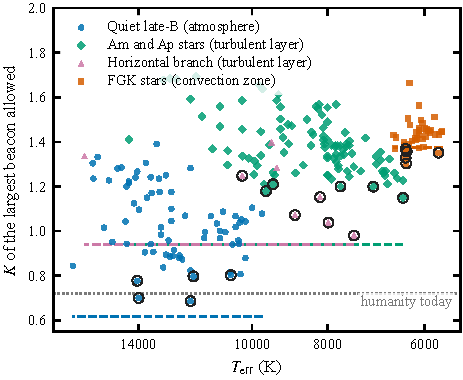
\includegraphics[width=\figwidth]{figures/archival.pdf}
\caption{Sagan type of the largest $^{99}$Tc beacon that the archival spectra of each star allow, against its effective temperature. Circles: quiet late-B hosts, whose Tc stays in the atmosphere. Diamonds: Am and Ap stars, and other stars hotter than 6400~K, which mix a turbulent layer. Triangles: horizontal-branch stars, given the same layer. Squares: metal-poor and normal dwarfs, which mix their convection zone. Dashed lines: the threshold of the representative host of each class at $S/N = 300$, across the temperatures of the class. Rings: the stars of Table~\ref{tab:archival}. Dotted line: humanity's power today.}
\label{fig:archival}
\end{figure}

Two metal-poor stars, HD~140283 and HD~84937, exclude the beacon that each would show at threshold, by 0.17~dex in abundance ($\Delta K = -0.02$). Their spectra hold so few metal lines that the \ion{Tc}{i} lines would fall on clean continuum. No quiet late-B star reaches its threshold. 3~Cen~A comes closest, at $\Delta K = +0.08$, and HD~175640 and HD~144667, both observed with STIS E230H, follow at $+0.11$, a factor of 13 in inventory. At $K \leq 0.69$ and 0.70, these two are the only stars whose spectra exclude a beacon that costs less than humanity's power. Among the stars that mix a turbulent layer the best is Vega, at $\Delta K = +0.15$, and the best horizontal-branch star, HD~161817, $+0.18$. Archival spectra of these stars fall short of $S/N = 300$, and blends count against Tc.

\subsection{A search for Tc lines}
\label{sec:archival_search}

A limit does not show that a star has no Tc below it. To check, we summed the absorption at the positions of each star's Tc lines, each weighted by its predicted strength over the noise, and compared the sum with the same sum after shifting the lines by trial velocities out to 300~km~s$^{-1}$. A star with Tc would stand out at zero velocity. Of 1039 such sums, one for each star, instrument and ion, none departs from the shifted sums by $4\sigma$, which chance alone would give 0.03 times. The two largest departures, $3.5\sigma$ in HD~144667 and in 46~Aql, come from the UVES \ion{Tc}{ii} lines at 3195, 3212 and 3237~\AA. Lines of \ion{Fe}{i}, \ion{V}{ii} and \ion{Co}{i} in the Kurucz lists fall within 3~km~s$^{-1}$ of all three \citep{Kurucz2011}. In HD~144667 the \ion{Tc}{ii} lines of the STIS spectrum limit Tc to $\log\epsilon_\mathrm{Tc} \leq 2.3$, while the UVES line at 3237~\AA\ alone allows 3.3, so the excess in the UVES spectrum is not Tc.

The clean-line statistic of Section~\ref{sec:blending} also gives upper limits in the same terms as a detection. For weak lines it grows in proportion to the abundance, so its $3\sigma$ limit lies $\log_{10}[(\max(z_0, 0) + 3)/5]$ above the $5\sigma$ detection, where $z_0$ is its value in the spectrum without Tc. These limits lie a median 0.6~dex above the limits of Section~\ref{sec:archival_method}. In HD~175640 the clean-line limit is $\log\epsilon \leq 2.3$, just below the detection at 2.4. The limits of Table~\ref{tab:archival} are therefore the more constraining, and they do not measure what a detection would need.

These limits share the limitations of Section~\ref{sec:limitations}, and two of them weigh more here. The limits in FGK stars rest on \ion{Tc}{i}, which overionization in non-LTE would weaken most in metal-poor stars, so these limits may be too deep. And the Fe abundances that set the opacity factor come from many analyses, whose solar Fe abundances differ by up to 0.2~dex.

\section{Discussion}
\label{sec:discussion}

\subsection{Cost}
\label{sec:cost}

Table~\ref{tab:beacons} compares the beacons. A photospheric beacon in a Sun-like star costs $6\times10^{19}$~W ($K = 1.37$), one in an Am star $2\times10^{15}$~W ($K = 0.94$), and one in the quiet late-B star $1.4\times10^{12}$~W ($K = 0.62$); the last two are read from space. Gas in front of the star costs less than the photospheric beacons of the Sun and the Am star, because every atom of it absorbs, whereas a photospheric beacon must fill the whole mixed layer of its star. A doped comet timed to transit the Am star costs $K = 0.99$, and an artificial comet around a Sun-like star costs $K = 0.71$. A photospheric beacon gives something in return. It is seen from every direction, and a $^{99}$Tc beacon lasts $10^{5}$~yr with no further effort, whereas a gas beacon is seen only from the directions chosen for it and must be renewed for as long as it runs. Among beacons seen from every direction, the photospheric beacon in an Am star is cheaper than a shell of gas ($K = 1.12$), but it needs a space telescope and rests on the uncertain mixed mass of A stars. A quiet late-B star that mixes nothing below its atmosphere costs $K = 0.62$, less than the artificial comet, but only if something holds the Tc in its atmosphere. If the Tc escapes, it costs $K = 1.06$ (Section~\ref{sec:levitation}). Read from the ground in the near-ultraviolet \ion{Tc}{ii} lines it costs $K = 0.75$. Without a space telescope, two other photospheric beacons also cost less than the sunlight intercepted by the Earth: the Am star read in the same lines ($K = 1.10$) and the late-B star read in \ion{Tc}{i} ($K = 1.09$).

\begin{table*}
\centering
\caption{Beacons of $^{99}$Tc bred from $^{98}$Mo, at $S/N = 300$ with the instruments listed: photospheric beacons (Section~\ref{sec:results}) and gas in front of the star (Section~\ref{sec:gas}). ``Sky'' is the fraction of the sky from which the beacon is seen; for a comet, the fraction from which it transits while it releases its dopant, near the plane of its orbit. Mass: the inventory of a photospheric beacon, and the dopant per event of a gas beacon. $K$ is the Sagan type of the upkeep of a photospheric beacon, and of the power that gives a monitoring program an even chance of catching a gas beacon in 10~yr, with 530 spectra a year from the ground or 20 from space.}
\label{tab:beacons}
\footnotesize
\begin{tabular}{lllrrr}
\toprule
Beacon & Host & Lines, telescope & Sky & Mass (kg) & $K$ \\
\midrule
Photosphere & Sun & Tc\,\textsc{i}, 8.2 m & 1 & $4.0\times10^{18}$ & 1.37 \\
Photosphere & Am star & Tc\,\textsc{ii}, 2.4 m space & 1 & $1.7\times10^{14}$ & 0.94 \\
Photosphere & Late B & Tc\,\textsc{ii}, 2.4 m space & 1 & $1.0\times10^{11}$ & 0.62 \\
\addlinespace
Comet, $\beta$~Pic-like & Am star & Tc\,\textsc{ii}, 2.4 m space & 0.045 & $2.8\times10^{10}$ & 1.20 \\
Comet, timed release & Am star & Tc\,\textsc{ii}, 2.4 m space & 0.045 & $1.9\times10^{8}$ & 0.99 \\
\addlinespace
Artificial comet & Sun & Tc\,\textsc{i}, 3.6 m & $1.2\times10^{-4}$ & $4.0\times10^{7}$ & 0.71 \\
Belt, $|b| < 3^\circ$ & Sun & Tc\,\textsc{i}, 3.6 m & 0.052 & $2.6\times10^{10}$ & 1.02 \\
Shell & Sun & Tc\,\textsc{i}, 3.6 m & 1 & $2.4\times10^{11}$ & 1.12 \\
\bottomrule
\end{tabular}

\end{table*}

A $^{99}$Tc beacon in a Sun-like star at the $S/N = 300$ threshold needs $4.0\times10^{18}$~kg of technetium. Making it by thermal fission of $^{235}$U takes $4.0\times10^{44}$ fissions. That burns $1.6\times10^{20}$~kg of $^{235}$U, $2.6\times10^{-5}\,\Mearth$, and releases $1.3\times10^{41}$~erg, about one year of the Sun's luminosity. Delivering the product into the star is cheap by comparison: a chemical rocket that cancels an orbital speed of 30~km~s$^{-1}$ puts $8\times10^{9}$~J into its exhaust for each kilogram delivered, $2.5\times10^{-6}$ of the fission energy per kilogram of Tc. The beacon then lasts $2\times10^{5}$~yr with no further effort. Bred from $^{98}$Mo instead, the same inventory takes $5.4\times10^{39}$~erg, 4 percent of a year of the Sun's output, and its upkeep is $5.6\times10^{19}$~W ($K = 1.37$). Either way it is a project for a civilization of the kind that \citet{Kardashev1964} imagined harnessing a large part of its star. Such energy-rich societies are also the ones whose technosignatures may be the most detectable and the least ambiguous \citep{Wright2022case}.

An Am-star host changes the picture. Its \ion{Tc}{ii} beacon needs $1.7\times10^{14}$~kg of $^{99}$Tc. Bred by neutron capture, that takes $2.3\times10^{35}$~erg, and the upkeep of $2.4\times10^{15}$~W ($K = 0.94$) is about 1 percent of the sunlight intercepted by the Earth and some 140 times humanity's primary power consumption in 2015, $1.7\times10^{13}$~W or $K = 0.72$ \citep{Gray2020}. In power this is a planetary-scale civilization, not a stellar one. In material it is more. Breeding the inventory fissions $2.8\times10^{14}$~kg of $^{235}$U, held in $4\times10^{16}$~kg of natural uranium, $7\times10^{-9}$ of the Earth's mass, unless breeder reactors fission $^{238}$U as well. It also takes $7\times10^{14}$~kg of natural molybdenum. The late-B beacon needs $2\times10^{13}$~kg of natural uranium.

A Pm beacon is cheaper to fill but expensive to keep. Harvested from fission products, the $5.4\times10^{17}$~kg of $^{147}$Pm in the Sun must be renewed at $1.4\times10^{17}$~kg~yr$^{-1}$, which takes fission power equal to 7 percent of the solar luminosity. Bred as $^{145}$Pm, which lives seven times longer and costs 65 times less per atom, the upkeep falls to $6\times10^{22}$~W, $1.6\times10^{-4}$ of the solar luminosity. In the M dwarf it is still 7 percent of the star's luminosity, and in the Am star $9\times10^{-8}$.

\subsection{Information in the signal}
\label{sec:signal}

A detection of either element in a main-sequence dwarf that is not chemically peculiar would be hard to explain naturally, and the two elements carry different information. A $^{99}$Tc beacon shows that technology existed at some time within the past $10^{5}$~yr; a $^{147}$Pm beacon shows that it is operating now, because the signal would vanish within a few decades without supply. The beacon also writes a record of its own history. $^{147}$Pm decays to $^{147}$Sm, so a promethium beacon in the Sun at threshold would double the solar samarium abundance ($\log\epsilon_\mathrm{Sm} = 0.96$; \citealt{Asplund2009}) in 260~yr and raise it by 0.7~dex in 1000~yr. A star with Pm and an excess of Sm in the ratio set by the half-life would show how long the beacon had run. Several nuclides together, Tc and Pm in a chosen ratio for instance, would add the kind of deliberately unnatural pattern that marks a signal as intentional.

The hosts that cost least, the A stars, are also those in which natural abundance anomalies are common. Am stars show large departures from solar abundances caused by diffusion \citep{Richer2000}, and the only claims of Tc and Pm in a main-sequence star concern the magnetic Ap star HD~101065 \citep{Cowley2000, Cowley2004, Fivet2007, Gopka2008} and similar objects \citep{Yushchenko2024}. None of these claims has been confirmed for Tc. In HD~101065 the absent resonance line limits it to $\log\epsilon_\mathrm{Tc} \leq 2.5$ \citep{Ryabchikova2008, Andrievsky2023tc}, and \citet{Yushchenko2024} report Pm in the hot peculiar star HD~25354 but only an upper limit for Tc, $\log\epsilon_\mathrm{Tc} < 4.0$. A civilization that wants to be recognized would therefore avoid magnetic Ap stars. Diffusion only redistributes elements that a star already contains, and an Am star has no reservoir of Tc or Pm to concentrate, so in a non-magnetic Am star these lines would still have no natural explanation. Spallation by accelerated particles at the stellar surface could make Tc \citep{Goriely2007}, and Galactic cosmic rays set a floor for it. Their energy density near the Sun, about 1.8~eV~cm$^{-3}$, is carried mostly by protons of a few GeV \citep{Ferriere2001}, a flux of about 30~cm$^{-2}$~s$^{-1}$. With a cross-section no larger than the geometric one of a Mo nucleus, 1~b, they keep $^{99}$Tc below $3\times10^{-10}$ of the Mo in a stellar atmosphere, or $\log\epsilon_\mathrm{Tc} < -7.6$ at the solar Mo abundance, six or more orders of magnitude below the thresholds of Section~\ref{sec:results}. The cheapest host is therefore also an acceptable one, although a beacon in a G or K dwarf would be even harder to dispute.

\subsection{Hosts beyond the main sequence}
\label{sec:wd}

We have modeled main-sequence hosts only. Two other classes are worth a comparison.

Red giants are poor hosts. As a star ascends the giant branch its convective envelope deepens in mass \citep{Karakas2014}, so a giant dilutes a pollutant in far more mass than a dwarf of the same temperature. Its beacon would cost more than the K dwarf's $K = 1.26$, and stars on the asymptotic giant branch make Tc themselves \citep{Merrill1952, Shetye2022}, so a Tc-rich giant has a natural explanation.

White dwarfs mix even less mass than A stars, but they do not keep it. In a DA white dwarf of $\log g = 8$ the convection zone contains $10^{-9}$ of the stellar mass at 8000~K, and heavy elements settle out of it in about $10^{3}$~yr; at 20{,}000~K it contains only $10^{-15.7}$ of the mass, and they settle in about a week \citep{Koester2009}. A white-dwarf beacon must therefore be fed continuously against settling, as debris from planetary systems is fed into the many white dwarfs in which metals are detected \citep{Koester2014}. Replacing the settling flux of a 0.6~$\Msun$ white dwarf by $^{99}$Tc bred from $^{98}$Mo takes an upkeep of $4.5\times10^{24}\,\epsilon_\mathrm{Tc}$~W at 20{,}000~K and $5.5\times10^{26}\,\epsilon_\mathrm{Tc}$~W at 8000~K, where $\epsilon_\mathrm{Tc}$ is the number abundance relative to hydrogen. To match the $K = 0.94$ of the Am star, the hot white dwarf would have to show Tc lines at $\log\epsilon_\mathrm{Tc} \leq 2.7$, and the cool one at $\log\epsilon_\mathrm{Tc} \leq 0.6$. We found no published search for Tc in a white dwarf. \citet{Werner2015} computed oscillator strengths for \ion{Tc}{iv}--\textsc{vi} so that it can be sought in hot post-AGB stars and (pre-)white dwarfs, where some Tc made on the asymptotic giant branch may survive; a Tc line in a young, hot white dwarf could therefore be natural. Our model atmospheres do not cover white dwarfs, so we cannot say whether their thresholds are that low. Because settling, not decay, sets the upkeep, bred Pm costs about the same per atom as bred Tc in a white dwarf, and a white-dwarf beacon is always a live one. White dwarfs are, however, far fainter than A stars, so the volume in which their beacons could be detected is much smaller.

\subsection{Lifetime and choice of host}
\label{sec:choice}

The cheapest hosts are short-lived. From their masses and luminosities, the late-B host burns its core hydrogen in roughly 0.2~Gyr and the Am host in roughly 1.5~Gyr, against 10~Gyr for the Sun. A technological species may never arise around a late-B star, and the A5--F2 range of \citet{Whitmire1980} raises the same question in a milder form. A civilization around a longer-lived star could instead pollute a conspicuous neighbor. Carrying the Tc to another star at 0.01~$c$ and stopping it there with a rocket of exhaust speed 0.03~$c$ costs 29 percent of the energy of breeding it, which raises $K$ by 0.01, and the journey takes 3000~yr for every 10~pc. The costs in this paper therefore apply to a nearby star of the builder's choosing as much as to its own.

\subsection{Distance reach}
\label{sec:horizon}

Figure~\ref{fig:horizon} shows the inventory that each instrument can detect in a 10~h exposure as a function of distance, with the photon-limited $S/N$ capped at 1000 to represent the systematic floor of a differential comparison (Section~\ref{sec:blending}). Close to the telescope the cap sets a floor. Beyond it the required inventory grows in proportion to distance, because the threshold equivalent width scales as $1/(S/N)$ and the photon-limited $S/N$ falls as $1/d$. For a Sun-like host the 8.2~m telescope stays at the floor out to 110~pc ($V = 10.1$) and the 39~m telescope out to 640~pc ($V = 13.8$). The Am host is brighter, and for it the 8.2~m and 39~m telescopes reach the floor out to 550~pc and 3.1~kpc. The \ion{Tc}{ii} ultraviolet beacon in the Am star is the cheapest of all but needs space. With an assumed efficiency of 1 percent, the 2.4~m ultraviolet echelle reaches the floor only out to 24~pc ($V = 4.0$); a 6~m space telescope with an efficiency of 5 percent would reach it out to 140~pc. Line blanketing removes 60 percent of the Am star's flux near 2543~\AA, which shortens these distances.

\begin{figure}[!tb]
\centering
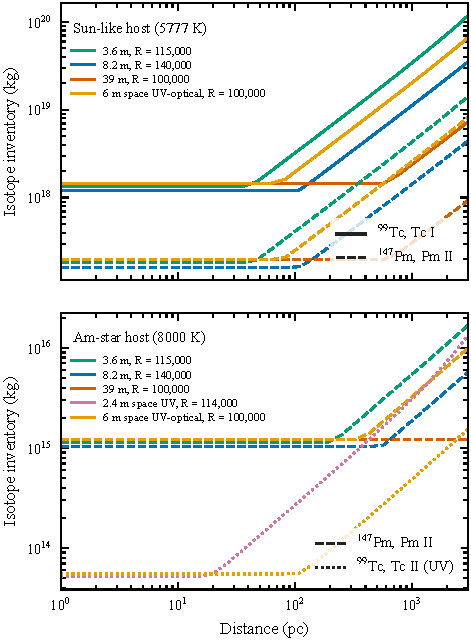
\includegraphics[width=\figwidth]{figures/horizon.pdf}
\caption{Inventory detected at $Z = 5$ in a 10~h exposure as a function of distance, for a Sun-like host (top) and an Am host (bottom). Colors denote instruments, line styles species: solid, \ion{Tc}{i} ($^{99}$Tc); dashed, \ion{Pm}{ii} ($^{147}$Pm); dotted, \ion{Tc}{ii} ultraviolet lines ($^{99}$Tc). The signal-to-noise ratio is photon-limited and capped at 1000 per pixel to represent the systematic floor of a differential comparison; the flat parts of the curves are that floor. The \ion{Tc}{i} beacon of the Am host needs more than $10^{17}$~kg and is not shown.}
\label{fig:horizon}
\end{figure}

\subsection{Reach on a human power budget}
\label{sec:budget_reach}

The thresholds of Section~\ref{sec:results} are for an observer who obtains $S/N = 300$, and so is close to the beacon. A civilization that spends more than the threshold upkeep holds more Tc, and its beacon is then seen at a lower $S/N$ and from farther away. We give the quiet late-B host of Section~\ref{sec:levitation}, assuming that its atmosphere holds the Tc, humanity's present power of $1.7\times10^{13}$~W \citep{Gray2020}. Bred by neutron capture, that holds $1.2\times10^{12}$~kg of $^{99}$Tc, 12 times the threshold inventory, which a 10~h exposure detects at $S/N = 31$ per pixel. Without dust, a 6~m space telescope would detect the beacon out to 23~kpc, and the 2.4~m telescope out to 4.2~kpc.

Dust limits this reach, because the \ion{Tc}{ii} lines lie near 2700~\AA, where the extinction is 2.1 times that in $V$ \citep{Gordon2023}. We placed stars by the Galaxy model of Section~\ref{sec:gas} and dust by the axisymmetric disk of \citet{DrimmelSpergel2001}, which gives $A_V = 0.57$~mag~kpc$^{-1}$ in the plane near the Sun. The 6~m telescope then detects the beacon from 9.1 percent of the Galaxy's stars, and from 18 or 4 percent with half or twice as much dust. The 339 star systems within 10~pc \citep{Reyle2021} and the local stellar density of $0.043\,\Msun$~pc$^{-3}$ \citep{McKee2015} give 1.9 systems per solar mass, so 9.1 percent is $1\times10^{10}$ systems. The 2.4~m telescope reaches 1.0 percent of the stars on the same budget, and the 6~m telescope reaches 0.4 percent at the threshold upkeep. A beacon fed at constant power fills over the decay time of $^{99}$Tc, and holds half its final inventory after $2.1\times10^{5}$~yr. After $10^{3}$~yr it holds 0.3 percent of that inventory, 0.04 of the threshold, which no receiver capped at $S/N = 1000$ detects. After $10^{4}$~yr it holds 0.4 of the threshold, which the 6~m telescope detects only within about 1~kpc.

A receiver that uses only the clean Tc lines would not detect this beacon at all. In HD~175640 such a receiver needs $\log\epsilon = 2.5$ at any $S/N$ above 30 (Section~\ref{sec:blending}), more than the 2.0 that humanity's power holds. With clean lines alone, the same reach takes about three times that power ($K = 0.77$).

A laser can reach the same number of stars at once, but at a far higher power. \citet{ClarkCahoy2018} take a laser to be noticed when it adds 0.1 percent to the light of its star in a 1~nm band, seen by a 1~m telescope, and find that 1~MW at 1315~nm sent through a 39~m aperture meets this from a Sun-like star to about 20{,}000 light years. Because the criterion is set by the star, a laser beside the late-B host must be brighter by the ratio of the two stars' luminosities at 1315~nm, which is 28 in the models of \citet{CastelliKurucz2003}. Lighting each of the $7.7\times10^{9}$ star systems within 5~kpc from that star takes 28~MW per system and $2\times10^{17}$~W in all ($K = 1.13$), $1.3\times10^{4}$ times humanity's power, and a transmitter for every system. From a Sun-like star it would take $8\times10^{15}$~W ($K = 0.99$). Humanity's power would light each system from the late-B host for only $8\times10^{-5}$ of the time, and an observer would have to look during that time. The Tc beacon is seen by as many systems on a budget $10^{4}$ times smaller, it shines in every direction, and it fades only with the half-life of $^{99}$Tc after its supply stops. In return it needs an ultraviolet spectrograph in space, it takes $10^{5}$~yr to fill, and it carries no message beyond its own existence. The comparison is also tilted in favor of the Tc beacon: its receiver is a 6~m ultraviolet spectrograph with a perfect model of the star, whereas the laser criterion assumes a 1~m photometric telescope.

\subsection{Search strategy}
\label{sec:search}

The \ion{Tc}{i} lines at 4238, 4262 and 4297~\AA\ and the strongest \ion{Pm}{ii} lines between 4138 and 5577~\AA\ lie within the coverage of the high-resolution spectrographs used for radial-velocity work, whose archives hold spectra of many nearby FGK stars. Searching such spectra needs no new telescope time, as the search of \citet{Tellis2017} for laser emission lines in the spectra of 5600 stars showed. Section~\ref{sec:archival} shows that archival spectra of metal-poor stars already reach the Sun-like threshold. Because the spectra of solar twins can be compared with one another line by line, a differential search of twins is the most sensitive version, and its floor will be set by how well two twins can be matched near 4300~\AA. A survey of $10^{5}$ stars in three ions with two instruments makes $6\times10^{5}$ trials, among which a $5\sigma$ excess occurs by chance 0.2 times. A detection in a single star must therefore be confirmed, by the other lines of the same species, by the second element, or at a second epoch.

A gas beacon is found differently. The \ion{Tc}{i} lines of an artificial comet are narrow, appear for about two months, and drift blueward during that time (Section~\ref{sec:gas}), so a search compares spectra of the same star taken at different epochs. The radial-velocity programs that monitor nearby Sun-like stars take many spectra of each target over years, and their archives can be searched for absorption at 4238, 4262 and 4297~\AA\ that is present in some epochs and absent in others. Doped natural comets can be sought now in the more than 9000 HARPS spectra of $\beta$~Pic \citep{Hoeijmakers2025}, as \ion{Ra}{ii} absorption at the velocities of the known Ca\,\textsc{ii} exocomet features.

\subsection{Limitations}
\label{sec:limitations}

The line formation is one-dimensional and in LTE. Departures from LTE in the ionization of Tc and Pm are likely; overionization of a minority neutral species in the upper photosphere of a solar-type star would weaken \ion{Tc}{i}, while \ion{Pm}{ii} and \ion{Tc}{ii}, the majority species in most hosts, are less affected. The oscillator strengths of Tc are uncertain by 0.15~dex \citep{Palmeri2005}, and those of Pm are theoretical \citep{Fivet2007}. The lines of other elements raise the thresholds by 0.06 to 0.28~dex (Section~\ref{sec:inventories}), and our ultraviolet synthesis of A and late-B stars makes \ion{Fe}{ii} lines 0.2 to 0.6~dex too weak at their measured abundances (Section~\ref{sec:validation}). The 3500~K ATLAS9 model lacks most molecular opacity, so the M-dwarf thresholds are the least reliable. The instrument efficiencies are assumed, and they affect only the distances of Section~\ref{sec:horizon}. The largest uncertainty, by far, is the mixed mass of the A stars, which spans five orders of magnitude in our model. The range that fits the abundances of Am stars is narrower and puts the Sagan type of the Am beacon between $K = 0.89$ and 0.99. The quiet late-B host rests on an assumed absence of mixing and on what happens to Tc at the top of its atmosphere, which no model yet follows. Every threshold assumes a receiver that knows the star's spectrum to the photon noise. Today's models of these stars fall far short of that in the ultraviolet, and a search that uses only the Tc lines on clean continuum needs about 40 times more Tc (Section~\ref{sec:blending}). The reach of Section~\ref{sec:budget_reach} uses an axisymmetric dust disk without spiral arms, which we bracket by halving and doubling it, and the laser comparison rests on one published design. The radiative support of Section~\ref{sec:levitation} is computed in LTE and for Tc only. The gas beacons of Section~\ref{sec:gas} rest on one well-measured comet and on the assumption that a comet's dopant is singly ionized. The photoionization rate of neutral Tc is borrowed from Mn, and the temperature at which a dispenser releases the gas, which sets how fast an artificial comet spreads, is assumed.

\section{Conclusions}
\label{sec:conclusions}

We have computed what a civilization must add to its star to make a beacon of technetium or promethium detectable with current high-resolution spectrographs, and compared it with gas placed in front of the star.
\begin{enumerate}
\item Our model confirms the argument of \citet{Whitmire1980} that early-type stars are the best photospheric hosts. Among hosts whose mixing is known from their abundances, the cheapest photospheric beacon is $^{99}$Tc in a non-magnetic Am star, whose turbulently mixed layer holds only about $10^{-5.5}$ of the stellar mass. Read in the \ion{Tc}{ii} ultraviolet lines by a 2.4~m space echelle, it needs $1.7\times10^{14}$~kg, and bred by neutron capture on $^{98}$Mo its upkeep is $2.4\times10^{15}$~W, $K = 0.94$. From the ground, the near-ultraviolet \ion{Tc}{ii} lines need $7\times10^{15}$~kg ($K = 1.10$). Radiation pushes Tc upward in A-star atmospheres 14 to 200 times harder than gravity, and even without that support Tc would take more than 50 half-lives to settle out of the mixed layer, so it stays until it decays. The mixing depths that fit the abundances of Am stars put $K$ between 0.89 and 0.99. A quiet late-B star that mixes nothing below its atmosphere costs $K = 1.06$, because radiation drives the Tc out of the atmosphere in 11~yr. If a weak, tangled magnetic field held it there, the beacon would cost $K = 0.62$ read from space and 0.75 read from the ground.
\item In a Sun-like star, with an 8~m-class telescope at $R = 140{,}000$ and $S/N = 300$, the \ion{Tc}{i} resonance lines reach a $5\sigma$ detection at $\log\epsilon_\mathrm{Tc} = +0.16$. That is $4\times10^{18}$~kg of $^{99}$Tc, with an upkeep of $K = 1.37$. None of the \ion{Tc}{i} lines is free of blends in the solar spectrum, so a search must be differential.
\item Breeding by neutron capture with fission neutrons costs at least 137~MeV per atom, 24 times less than harvesting $^{99}$Tc from fission products and 65 times less than $^{147}$Pm. Promethium beacons still cost $K \geq 1.31$, because even bred $^{145}$Pm must be replaced every few decades. In return a Pm beacon shows that its builder is active now, and its decay product samarium records how long it has run.
\item Red giants are worse hosts than dwarfs. White dwarfs, fed against settling, could rival the Am star if their Tc threshold is $\log\epsilon_\mathrm{Tc} \leq 2.7$ at 20{,}000~K, but they are faint and remain to be modeled.
\item On humanity's present power, $1.7\times10^{13}$~W, the quiet late-B beacon, if its atmosphere held the Tc, would hold 12 times its threshold inventory. Once it had filled, after some $10^{5}$~yr, a receiver with a 6~m ultraviolet space telescope that knew the star's spectrum to the photon noise would detect it through the Galaxy's dust from about a tenth of the Galaxy's star systems, $10^{10}$ of them. A receiver that used only the clean Tc lines would need three times that power, and after $10^{3}$~yr of filling the beacon is not yet detectable. Lighting the $8\times10^{9}$ systems within 5~kpc with lasers from the same star, which must outshine it, would take $10^{4}$ times more power.
\item Gas in front of the star needs far less material, because every atom absorbs. A comet doped with $^{99}$Tc and timed to transit an Am star costs $K = 0.99$, and \ion{Ra}{ii} is the most sensitive dopant of such a comet. A cloud of neutral $^{99}$Tc released at rest in front of a Sun-like star, which radiation pressure keeps on the disk, costs $1.3\times10^{13}$~W ($K = 0.71$) for an even chance of detection in 10~yr. Such a cloud is aimed at one target. A belt in the Galactic plane that reaches three quarters of the Galaxy's stars costs $K = 1.02$, and a shell $K = 1.12$.
\item Archival spectra of 222 stars show no Tc. Two metal-poor stars, HD~140283 and HD~84937, exclude by 0.17~dex the beacon that each would show at threshold in its own model. The best quiet late-B hosts come within a factor of 10 to 13 of their own thresholds. A detection needs more than an exclusion. With today's models a search must use only the Tc lines on clean continuum, and in HD~175640 it then needs 40 times the ideal inventory.
\end{enumerate}
The archives of radial-velocity programs already hold high-resolution spectra of many nearby Sun-like stars, in which a photospheric beacon can be sought differentially among solar twins and a gas beacon from one epoch to the next.

\begin{acknowledgments}
We thank R.~L.~Kurucz for making the ATLAS9 model atmospheres, the atomic line lists and the Kitt Peak solar flux atlas freely available, and E.~Mamajek for maintaining the dwarf-star sequence used here. This research has made use of NASA's Astrophysics Data System and the SciX digital library, the NIST Atomic Spectra Database, and the IAEA Live Chart of Nuclides.

This research is based on observations made with the NASA/ESA Hubble Space Telescope obtained from the Space Telescope Science Institute, which is operated by the Association of Universities for Research in Astronomy, Inc., under NASA contract NAS5--26555, associated with programs 1064, 1182, 2461, 2800, 3125, 3207, 3372, 3479, 3496, 3961, 4510, 4766, 4808, 5598, 5693, 5855, 5860, 5862, 5869, 6087, 6213, 6245, 6275, 6534, 7348, 7402, 8197, 8770, 9048, 9146, 9455, 9491, 9804, 9848, 9900, 9974, 12023, 12981, 13346, 14161, 14672, 14767, 15139, 15179, 16086, 17184, 18104; on observations made with the International Ultraviolet Explorer, obtained from the MAST data archive at the Space Telescope Science Institute; on data obtained from the ESO Science Archive Facility with DOIs \url{https://doi.org/10.18727/archive/33}, \url{https://doi.org/10.18727/archive/50}, \url{https://doi.org/10.18727/archive/21}, \url{https://doi.org/10.18727/archive/24}, \url{https://doi.org/10.18727/archive/25}; on observations obtained at the Canada-France-Hawai{\textquoteleft}i Telescope (CFHT), which is operated by the National Research Council of Canada, the Institut National des Sciences de l'Univers of the Centre National de la Recherche Scientifique of France, and the University of Hawai{\textquoteleft}i; on spectral data retrieved from the ELODIE archive at Observatoire de Haute-Provence (OHP) \citep{Moultaka2004}; and on data retrieved from the SOPHIE archive at OHP, available at \url{http://atlas.obs-hp.fr/sophie}. CFHT is located on Maunakea on Hawai{\textquoteleft}i Island, a mountain of considerable cultural, natural, and ecological significance. Maunakea is a sacred site to Native Hawaiians, also known as K\={a}naka {\textquoteleft}\={O}iwi. Quality observations are made possible by relentless effort of the entire staff at Canada-France-Hawai{\textquoteleft}i Telescope. This research used the facilities of the Canadian Astronomy Data Centre operated by the National Research Council of Canada with the support of the Canadian Space Agency. The ESPaDOnS and Narval spectra were reduced with Libre-ESpRIT \citep{Donati1997}, and some were obtained from PolarBase \citep{Petit2014}. This work has made use of data from the European Space Agency (ESA) mission {\it Gaia} (\url{https://www.cosmos.esa.int/gaia}), processed by the {\it Gaia} Data Processing and Analysis Consortium (DPAC, \url{https://www.cosmos.esa.int/web/gaia/dpac/consortium}). Funding for the DPAC has been provided by national institutions, in particular the institutions participating in the {\it Gaia} Multilateral Agreement \citep{GaiaCollaboration2016, GaiaCollaboration2023}. This research has made use of the SIMBAD database, operated at CDS, Strasbourg, France \citep{Wenger2000}, and of the VizieR catalogue access tool, CDS, Strasbourg, France (DOI: 10.26093/cds/vizier; \citealt{Ochsenbein2000}).

The code, input tables, figure scripts and manuscript source are in the repository that accompanies this paper. We take full responsibility for the contents of this paper. We used large language models (Claude), under our supervision, to search the literature, to write the line-formation, detection and figure scripts, to draft and edit the text, and to refine the figures. The figures are produced by those scripts; no generative model created or altered plotted data. Every bibliography entry was exported from the NASA Astrophysics Data System.
\end{acknowledgments}

\appendix

\section{Line list}
\label{app:lines}

Table~\ref{tab:lines} lists the lines of Sections~\ref{sec:threshold} and~\ref{sec:archival}. Wavelengths are in air, and $\chi$ is the energy of the lower level. Oscillator strengths of Tc are from \citet{Kurucz2011} and those of Pm from \citet{Fivet2007}.

\begin{table*}
\centering
\caption{Lines used. t: in the detection statistic of Section~\ref{sec:threshold}. a: sets the archival limit of at least one star (Section~\ref{sec:archival}).}
\label{tab:lines}
\footnotesize
\setlength{\tabcolsep}{3pt}
\iftwocol\begin{tabular}{rrrl@{\hspace{10pt}}rrrl@{\hspace{10pt}}rrrl}
\toprule
\multicolumn{4}{c}{Tc\,\textsc{i}} & \multicolumn{4}{c}{Tc\,\textsc{ii}} & \multicolumn{4}{c}{Pm\,\textsc{ii}} \\
\cmidrule(lr){1-4}\cmidrule(lr){5-8}\cmidrule(lr){9-12}
$\lambda$ (\AA) & $\chi$ (eV) & $\log gf$ & Use & $\lambda$ (\AA) & $\chi$ (eV) & $\log gf$ & Use & $\lambda$ (\AA) & $\chi$ (eV) & $\log gf$ & Use \\
\midrule
2509.81 & 0.00 & $-1.575$ & a & 2285.46 & 0.00 & $-1.364$ & a & 4137.95 & 0.37 & $+0.300$ & t \\
3636.07 & 0.32 & $+0.443$ & a & 2298.09 & 0.00 & $-0.909$ & t & 4157.86 & 0.25 & $+0.360$ & t \\
3726.35 & 0.46 & $-0.312$ & a & 2496.77 & 0.43 & $-0.032$ & t & 4186.03 & 0.14 & $+0.320$ & t \\
3746.85 & 0.46 & $+0.081$ & a & 2529.34 & 0.52 & $-0.339$ & t & 4216.31 & 0.06 & $-0.060$ & t \\
3984.97 & 0.32 & $-0.162$ & a & 2543.22 & 0.00 & $+0.494$ & ta & 4297.78 & 0.00 & $+0.080$ & t \\
4031.62 & 0.32 & $+0.308$ & a & 2544.82 & 0.52 & $-0.619$ & t & 4325.92 & 0.50 & $-0.540$ & t \\
4095.66 & 0.40 & $-0.102$ & a & 2547.93 & 0.58 & $-0.784$ & t & 4332.05 & 0.37 & $-0.580$ & t \\
4170.27 & 0.52 & $-0.670$ & a & 2558.60 & 0.58 & $-0.523$ & t & 4340.53 & 0.25 & $-0.370$ & t \\
4238.18 & 0.00 & $-0.436$ & t & 2567.03 & 0.62 & $-0.655$ & t & 4342.12 & 0.14 & $-0.900$ & t \\
4262.24 & 0.00 & $-0.233$ & ta & 2610.00 & 0.00 & $+0.354$ & ta & 4381.88 & 0.06 & $-0.710$ & t \\
4297.03 & 0.00 & $-0.071$ & ta & 2634.91 & 2.98 & $+0.707$ & t & 4432.51 & 0.20 & $-0.700$ & t \\
5096.27 & 1.30 & $-0.323$ & a & 2643.01 & 2.97 & $+0.524$ & t & 4500.15 & 0.47 & $-1.890$ & t \\
5161.81 & 1.64 & $-0.472$ & a & 2647.01 & 0.00 & $+0.212$ & ta & 4508.59 & 0.25 & $-2.330$ & t \\
5174.81 & 1.37 & $-0.753$ & a & 2652.35 & 2.98 & $+0.603$ & t & 4517.92 & 0.14 & $-2.680$ & t \\
5375.20 & 3.73 & $+0.703$ & a & 2665.73 & 2.97 & $+0.320$ & t & 4525.20 & 0.62 & $-0.730$ & t \\
 & & &  & 2670.82 & 2.97 & $-0.555$ & t & 4530.72 & 0.37 & $-1.450$ & t \\
 & & &  & 2673.41 & 2.98 & $-0.616$ & t & 4538.53 & 0.50 & $-1.670$ & t \\
 & & &  & 2675.22 & 2.97 & $-0.167$ & t & 4615.87 & 0.20 & $-0.760$ & t \\
 & & &  & 2682.70 & 2.97 & $-0.913$ & t & 4651.93 & 0.33 & $-0.670$ & t \\
 & & &  & 2684.23 & 2.98 & $+0.330$ & ta & 4714.91 & 0.47 & $-1.760$ & t \\
 & & &  & 2686.03 & 2.98 & $-0.111$ & t & 4758.36 & 0.62 & $-2.370$ & t \\
 & & &  & 2688.03 & 2.96 & $-0.835$ & t & 4854.30 & 0.33 & $-1.920$ & t \\
 & & &  & 2693.74 & 2.97 & $-0.302$ & t & 4913.87 & 0.47 & $-1.150$ & t \\
 & & &  & 2711.48 & 2.96 & $-0.234$ & t & 4981.32 & 0.87 & $-2.610$ & t \\
 & & &  & 2724.19 & 2.96 & $-0.311$ & t & 5024.71 & 0.76 & $-2.100$ & t \\
 & & &  & 2725.65 & 2.97 & $-0.349$ & t & 5079.03 & 0.66 & $-2.690$ & t \\
 & & &  & 2730.05 & 2.97 & $-0.832$ & t & 5242.83 & 1.00 & $-1.040$ & t \\
 & & &  & 2730.23 & 2.97 & $-0.315$ & t & 5265.32 & 0.87 & $-2.540$ & t \\
 & & &  & 2733.68 & 2.98 & $+0.065$ & t & 5293.92 & 0.76 & $-0.970$ & t \\
 & & &  & 2734.65 & 2.97 & $-0.442$ & t & 5310.65 & 0.66 & $-1.410$ & t \\
 & & &  & 2795.78 & 2.98 & $+0.553$ & t & 5520.67 & 0.75 & $-3.580$ & t \\
 & & &  & 2809.65 & 2.98 & $-0.083$ & t & 5546.08 & 0.76 & $-0.260$ & t \\
 & & &  & 2811.61 & 2.98 & $+0.361$ & t & 5556.88 & 1.13 & $-0.030$ & t \\
 & & &  & 2821.35 & 2.97 & $+0.266$ & t & 5558.39 & 1.00 & $-0.940$ & t \\
 & & &  & 2825.04 & 2.98 & $-0.160$ & t & 5561.73 & 0.87 & $-0.040$ & t \\
 & & &  & 2831.18 & 2.97 & $+0.104$ & t & 5576.02 & 0.66 & $-0.170$ & t \\
 & & &  & 2836.12 & 2.97 & $-0.279$ & t & 5670.61 & 0.70 & $-3.080$ & t \\
 & & &  & 2840.37 & 2.96 & $-0.055$ & t & 6075.09 & 0.95 & $-3.280$ & t \\
 & & &  & 2846.75 & 2.97 & $-0.574$ & t & 6152.74 & 0.87 & $-3.180$ & t \\
 & & &  & 3195.21 & 1.56 & $-0.101$ & ta & 6424.87 & 0.95 & $-3.160$ & t \\
 & & &  & 3212.01 & 1.56 & $+0.098$ & t &  & & &  \\
 & & &  & 3237.01 & 1.56 & $+0.233$ & ta &  & & &  \\
 & & &  & 3892.13 & 1.56 & $-1.145$ & a &  & & &  \\
 & & &  & 3975.02 & 1.56 & $-1.628$ & a &  & & &  \\
\bottomrule
\end{tabular}
\else\scriptsize\resizebox{\textwidth}{!}{\begin{tabular}{rrrl@{\hspace{10pt}}rrrl@{\hspace{10pt}}rrrl}
\toprule
\multicolumn{4}{c}{Tc\,\textsc{i}} & \multicolumn{4}{c}{Tc\,\textsc{ii}} & \multicolumn{4}{c}{Pm\,\textsc{ii}} \\
\cmidrule(lr){1-4}\cmidrule(lr){5-8}\cmidrule(lr){9-12}
$\lambda$ (\AA) & $\chi$ (eV) & $\log gf$ & Use & $\lambda$ (\AA) & $\chi$ (eV) & $\log gf$ & Use & $\lambda$ (\AA) & $\chi$ (eV) & $\log gf$ & Use \\
\midrule
2509.81 & 0.00 & $-1.575$ & a & 2285.46 & 0.00 & $-1.364$ & a & 4137.95 & 0.37 & $+0.300$ & t \\
3636.07 & 0.32 & $+0.443$ & a & 2298.09 & 0.00 & $-0.909$ & t & 4157.86 & 0.25 & $+0.360$ & t \\
3726.35 & 0.46 & $-0.312$ & a & 2496.77 & 0.43 & $-0.032$ & t & 4186.03 & 0.14 & $+0.320$ & t \\
3746.85 & 0.46 & $+0.081$ & a & 2529.34 & 0.52 & $-0.339$ & t & 4216.31 & 0.06 & $-0.060$ & t \\
3984.97 & 0.32 & $-0.162$ & a & 2543.22 & 0.00 & $+0.494$ & ta & 4297.78 & 0.00 & $+0.080$ & t \\
4031.62 & 0.32 & $+0.308$ & a & 2544.82 & 0.52 & $-0.619$ & t & 4325.92 & 0.50 & $-0.540$ & t \\
4095.66 & 0.40 & $-0.102$ & a & 2547.93 & 0.58 & $-0.784$ & t & 4332.05 & 0.37 & $-0.580$ & t \\
4170.27 & 0.52 & $-0.670$ & a & 2558.60 & 0.58 & $-0.523$ & t & 4340.53 & 0.25 & $-0.370$ & t \\
4238.18 & 0.00 & $-0.436$ & t & 2567.03 & 0.62 & $-0.655$ & t & 4342.12 & 0.14 & $-0.900$ & t \\
4262.24 & 0.00 & $-0.233$ & ta & 2610.00 & 0.00 & $+0.354$ & ta & 4381.88 & 0.06 & $-0.710$ & t \\
4297.03 & 0.00 & $-0.071$ & ta & 2634.91 & 2.98 & $+0.707$ & t & 4432.51 & 0.20 & $-0.700$ & t \\
5096.27 & 1.30 & $-0.323$ & a & 2643.01 & 2.97 & $+0.524$ & t & 4500.15 & 0.47 & $-1.890$ & t \\
5161.81 & 1.64 & $-0.472$ & a & 2647.01 & 0.00 & $+0.212$ & ta & 4508.59 & 0.25 & $-2.330$ & t \\
5174.81 & 1.37 & $-0.753$ & a & 2652.35 & 2.98 & $+0.603$ & t & 4517.92 & 0.14 & $-2.680$ & t \\
5375.20 & 3.73 & $+0.703$ & a & 2665.73 & 2.97 & $+0.320$ & t & 4525.20 & 0.62 & $-0.730$ & t \\
 & & &  & 2670.82 & 2.97 & $-0.555$ & t & 4530.72 & 0.37 & $-1.450$ & t \\
 & & &  & 2673.41 & 2.98 & $-0.616$ & t & 4538.53 & 0.50 & $-1.670$ & t \\
 & & &  & 2675.22 & 2.97 & $-0.167$ & t & 4615.87 & 0.20 & $-0.760$ & t \\
 & & &  & 2682.70 & 2.97 & $-0.913$ & t & 4651.93 & 0.33 & $-0.670$ & t \\
 & & &  & 2684.23 & 2.98 & $+0.330$ & ta & 4714.91 & 0.47 & $-1.760$ & t \\
 & & &  & 2686.03 & 2.98 & $-0.111$ & t & 4758.36 & 0.62 & $-2.370$ & t \\
 & & &  & 2688.03 & 2.96 & $-0.835$ & t & 4854.30 & 0.33 & $-1.920$ & t \\
 & & &  & 2693.74 & 2.97 & $-0.302$ & t & 4913.87 & 0.47 & $-1.150$ & t \\
 & & &  & 2711.48 & 2.96 & $-0.234$ & t & 4981.32 & 0.87 & $-2.610$ & t \\
 & & &  & 2724.19 & 2.96 & $-0.311$ & t & 5024.71 & 0.76 & $-2.100$ & t \\
 & & &  & 2725.65 & 2.97 & $-0.349$ & t & 5079.03 & 0.66 & $-2.690$ & t \\
 & & &  & 2730.05 & 2.97 & $-0.832$ & t & 5242.83 & 1.00 & $-1.040$ & t \\
 & & &  & 2730.23 & 2.97 & $-0.315$ & t & 5265.32 & 0.87 & $-2.540$ & t \\
 & & &  & 2733.68 & 2.98 & $+0.065$ & t & 5293.92 & 0.76 & $-0.970$ & t \\
 & & &  & 2734.65 & 2.97 & $-0.442$ & t & 5310.65 & 0.66 & $-1.410$ & t \\
 & & &  & 2795.78 & 2.98 & $+0.553$ & t & 5520.67 & 0.75 & $-3.580$ & t \\
 & & &  & 2809.65 & 2.98 & $-0.083$ & t & 5546.08 & 0.76 & $-0.260$ & t \\
 & & &  & 2811.61 & 2.98 & $+0.361$ & t & 5556.88 & 1.13 & $-0.030$ & t \\
 & & &  & 2821.35 & 2.97 & $+0.266$ & t & 5558.39 & 1.00 & $-0.940$ & t \\
 & & &  & 2825.04 & 2.98 & $-0.160$ & t & 5561.73 & 0.87 & $-0.040$ & t \\
 & & &  & 2831.18 & 2.97 & $+0.104$ & t & 5576.02 & 0.66 & $-0.170$ & t \\
 & & &  & 2836.12 & 2.97 & $-0.279$ & t & 5670.61 & 0.70 & $-3.080$ & t \\
 & & &  & 2840.37 & 2.96 & $-0.055$ & t & 6075.09 & 0.95 & $-3.280$ & t \\
 & & &  & 2846.75 & 2.97 & $-0.574$ & t & 6152.74 & 0.87 & $-3.180$ & t \\
 & & &  & 3195.21 & 1.56 & $-0.101$ & ta & 6424.87 & 0.95 & $-3.160$ & t \\
 & & &  & 3212.01 & 1.56 & $+0.098$ & t &  & & &  \\
 & & &  & 3237.01 & 1.56 & $+0.233$ & ta &  & & &  \\
 & & &  & 3892.13 & 1.56 & $-1.145$ & a &  & & &  \\
 & & &  & 3975.02 & 1.56 & $-1.628$ & a &  & & &  \\
\bottomrule
\end{tabular}
}\fi
\end{table*}

\software{\texttt{numpy} \citep{Harris2020}, \texttt{scipy} \citep{Virtanen2020}, \texttt{matplotlib} \citep{Hunter2007}.}
%% ---- END BODY ----

\section*{Declaration of competing interest}
The author declares no competing financial interests or personal relationships that could have appeared to influence the work reported in this paper.

\section*{CRediT authorship contribution statement}
\textbf{James Guillochon:} Conceptualization, Methodology, Software, Formal analysis, Investigation, Visualization, Writing -- original draft, Writing -- review \& editing.

\section*{Declaration of generative AI and AI-assisted technologies in the writing process}
During the preparation of this work the author used Claude (Anthropic) to search the literature, write analysis code, and draft and edit the text. After using this tool, the author reviewed and edited the content as needed and takes full responsibility for the content of the publication.

\section*{Data availability}
All inputs are public: the ATLAS9 model atmospheres, Kurucz's line lists and solar flux atlas, the \ion{Pm}{ii} data of Fivet et al., the IAEA and NIST databases, and the archival spectra of Section~\ref{sec:archival}, from the ESO Science Archive, MAST, the Canadian Astronomy Data Centre, the Observatoire de Haute-Provence and PolarBase. The parameters, sources and limits of the 222 stars are in the machine-readable table \texttt{archival\_limits.csv}, the clean-line detection thresholds of every archival spectrum in \texttt{detect.csv}, and the Tc lines that the limits use in \texttt{tc\_lines.csv}. The code and derived tables are available in the repository that accompanies this paper.

\bibliographystyle{elsarticle-num-names}
\bibliography{references}

\end{document}
